\documentclass[11pt,a4paper]{article}
\usepackage[margin=2.4cm]{geometry}
\usepackage{amsmath,amssymb,amsthm}
\usepackage{booktabs,array,longtable}
\usepackage{enumitem}
\usepackage{float}
\usepackage[hidelinks]{hyperref}
\usepackage{tikz}
\usetikzlibrary{positioning,arrows.meta}
\usepackage{pgfplots}
\pgfplotsset{compat=1.16}

\newtheorem{theorem}{Theorem}
\newtheorem{lemma}[theorem]{Lemma}
\newtheorem{corollary}[theorem]{Corollary}
\newtheorem{proposition}[theorem]{Proposition}
\theoremstyle{definition}
\newtheorem{definition}[theorem]{Definition}
\newtheorem{example}[theorem]{Example}
\newtheorem{remark}[theorem]{Remark}

\newcommand{\Fix}{\operatorname{Fix}}
\newcommand{\code}[1]{\texttt{#1}}
\newcommand{\ALO}{\operatorname{ALO}}
\newcommand{\AMO}{\operatorname{AMO}}
\newcommand{\EO}{\operatorname{EO}}
\newcommand{\st}[1]{\textsf{#1}}
\setlist{itemsep=2pt,topsep=4pt}
\setlist[description]{font=\normalfont}

% Corresponding author.
\newcommand{\AuthorName}{Charles Gretton}
\newcommand{\AuthorEmail}{\href{mailto:charles.gretton@anu.edu.au}{charles.gretton@anu.edu.au}}

\title{Transpose-Symmetric Costas Arrays of Order 32:\\
An Independent Verification by Fixed-Point Decomposition and Distributed SAT\\[4pt]
\large Report, revision 16}
\author{\AuthorName\thanks{Corresponding author: \AuthorEmail.}\\ Costas-32 project}
\date{18 October 2026}

\begin{document}
\maketitle

\begin{center}\begin{minipage}{0.9\textwidth}\small
\noindent\textbf{Licence.} \textcopyright\ 2026 Charles Gretton. This report is licensed under the Creative Commons Attribution 4.0 International licence (CC BY 4.0).
To view a copy of the licence, visit \url{https://creativecommons.org/licenses/by/4.0/}. The software released
with it in the Costas-32 repository is licensed under the Apache License, Version 2.0
(\url{https://www.apache.org/licenses/LICENSE-2.0}). Material by others that is cited or reproduced here,
including published data and catalogues, remains under its original terms.

\smallskip\noindent\textbf{Errata.} We welcome reports of errors, omissions and overlooked prior work. Please send them to the
corresponding author, Charles Gretton, at \href{mailto:charles.gretton@anu.edu.au}{charles.gretton@anu.edu.au}.
Every report that leads to a correction will be acknowledged in the errata and in any revised edition,
cited as a private communication; where the point was already made in a publication that appeared before
this report's publication date, that publication will be cited as well.
\end{minipage}\end{center}

\begin{abstract}
A Costas array is a permutation matrix in which no two pairs of dots are separated by the
same vector. No Costas array of order 32 is known, and order 32 is the smallest order for
which existence is open. This report studies the arrays that are symmetric about their main
diagonal, which correspond to permutations that are their own inverse. Their non-existence at
order 32 is already known: exhaustive enumerations of symmetric Costas arrays, published in
1993 through order 32 and extended in 2009 to order 36, find none of order 32. We verify it independently, by an entirely different method: a complete
search built on a new decomposition.
The search rests on a decomposition. The fixed points of such an array form a Golomb ruler,
so there are 0, 2, 4 or 6 of them, and up to reflection the problem splits into
44{,}947 disjoint regions, one per fixed-point set. Each region is encoded exactly
as a SAT instance. Easy regions were decided by the solver Kissat on one core each; hard
regions by the distributed solver Dagster on a 104-core node, using a native split
whose split coordinates are chosen so that the fixed points refute the subproblems that
would otherwise dominate the run. The single region with no fixed points was decided by a
further case split on one transposition, with reflection symmetry breaking. All 44{,}947
regions received UNSAT verdicts and none produced a validated solution; the listed production
runs used 16{,}887 service units in our HPC environment. The verification is computational, under explicit trust assumptions: the negative verdicts
are solver results, not yet supported by checked proof certificates. Its main interest is
methodological: it shows how the structure of a combinatorial problem can drive the
decomposition of its hardest parts.
\end{abstract}

\section*{Contributions}
\addcontentsline{toc}{section}{Contributions}

This report asks whether a \emph{Costas array} of order 32 can be symmetric about its main diagonal.
The literature has answered it in the negative, by exhaustive enumeration in 1993 and again in
2009 (Section~\ref{sec:censuses}). We answer it again, independently and by a different method,
whose design is the main subject of the report. Its contributions are as follows.

\begin{enumerate}
\item We observe that the \emph{fixed points} of a \emph{transpose-symmetric} Costas array form a \emph{Golomb ruler},
and use this to partition the order-32 problem into 44{,}947 disjoint \emph{regions}, one for each
\emph{reflection-canonical} set of fixed points (Section~\ref{sec:framework}).
\item We encode each region as a satisfiability problem whose edge-variable projections are
exactly the Costas \emph{involutions} with the region's fixed points. The encoding is proved exact and
validated exhaustively at small orders (Section~\ref{sec:encoding}).
\item We introduce a \emph{native split} for the distributed solver Dagster, in which a source vertex
enumerates the partners of a few chosen coordinates. The coordinates are chosen so that the fixed
points refute every \emph{unsplit branch}, the one kind of subproblem that otherwise dominates a run.
We prove the decomposition exhaustive, and show empirically that this choice governs its
performance (Sections~\ref{sec:decomp} and~\ref{sec:lessons}).
\item For the one region without fixed points, we fix a single \emph{transposition}, which then plays
the role of the fixed points, and add reflection \emph{symmetry breaking} (Section~\ref{sec:cases}).
\item We report a complete campaign in our HPC environment in which all 44{,}947 regions are
search-closed. This independently confirms, by a method sharing no software or approach with the
earlier enumerations, that no transpose-symmetric Costas array of order 32 exists, and hence none invariant
under any non-identity symmetry of the square. The
verdicts are uncertified solver results under stated trust assumptions, and every distributed
closure passes a message-accounting audit (Sections~\ref{sec:results} and~\ref{sec:claim}).
\end{enumerate}

Structural theorems obtained earlier in this project had excluded every candidate with at most
one \emph{large-large} pair (Section~\ref{sec:earlier}); the campaign completes that line
independently. The work concerns the symmetric subclass only. Whether any Costas array of order
32 exists remains open.

\begin{figure}[H]
\centering
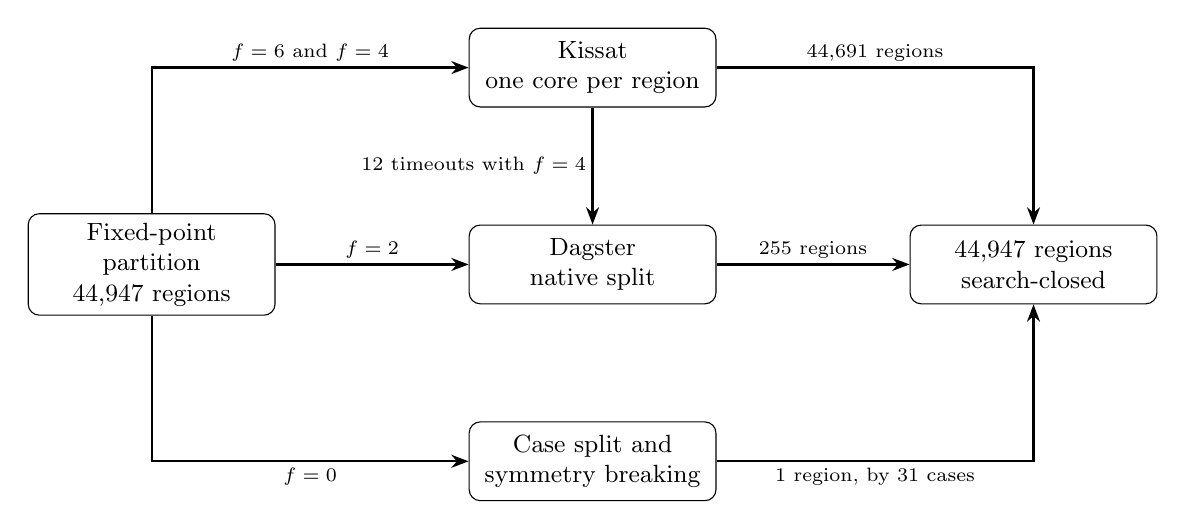
\begin{tikzpicture}[every node/.style={font=\small},
  box/.style={draw, rounded corners, align=center, minimum height=10mm, text width=29mm},
  arr/.style={-{Stealth[length=2.2mm]}, thick}, lab/.style={font=\scriptsize, inner sep=2pt}]
\node[box] (enum) at (0,0) {Fixed-point partition\\44{,}947 regions};
\node[box] (k)  at (5.6, 2.5) {Kissat\\one core per region};
\node[box] (d)  at (5.6, 0) {Dagster\\native split};
\node[box] (c)  at (5.6,-2.5) {Case split and\\symmetry breaking};
\node[box] (done) at (11.2,0) {44{,}947 regions\\search-closed};
\draw[arr] (enum.north) |- node[lab, pos=0.75, above]{$f=6$ and $f=4$} (k.west);
\draw[arr] (enum.east) -- node[lab, above]{$f=2$} (d.west);
\draw[arr] (enum.south) |- node[lab, pos=0.75, below]{$f=0$} (c.west);
\draw[arr] (k.south) -- node[lab, left]{12 timeouts with $f=4$} (d.north);
\draw[arr] (k.east) -| node[lab, pos=0.25, above]{44{,}691 regions} (done.north);
\draw[arr] (d.east) -- node[lab, above]{255 regions} (done.west);
\draw[arr] (c.east) -| node[lab, pos=0.25, below]{1 region, by 31 cases} (done.south);
\end{tikzpicture}
\caption{The campaign. Regions with six or four fixed points were run with Kissat, and the 12
it left open after an hour went to Dagster. The 256 regions with two fixed points went to Dagster,
apart from the 13 that Kissat had already closed within four hours in the sample. The region with
no fixed points was case-split first. Numbers on the right are regions closed by each route.}
\label{fig:pipeline}
\end{figure}


\tableofcontents

\section*{Glossary and status vocabulary}
\addcontentsline{toc}{section}{Glossary and status vocabulary}
\begin{description}[style=nextline, leftmargin=2.6cm, itemsep=1pt]
\item[displacement] the vector $(j-i,\pi(j)-\pi(i))$ between the dots of columns $i<j$
\item[involution] a permutation equal to its inverse; a transposition $(a\,b)$ swaps $a,b$
\item[fixed point] a coordinate $c$ with $\pi(c)=c$, a dot on the main diagonal
\item[region] the set $R_F$ of Costas involutions with fixed-point set exactly $F$
\item[free coordinate] a coordinate not in $F$; the set of them is $V$
\item[edge variable] $x_{ab}$, true when the transposition $(a\,b)$ is present
\item[message] a subproblem sent by Dagster: an assignment of partners to split coordinates
\item[unsplit branch] a message in which two split coordinates are paired with each other
\item[seed-refuted] a pairing that repeats a displacement with the fixed dots alone
\item[case] a region with one transposition fixed, written \code{R00000@0-}$x$
\end{description}

\noindent Verdicts: \st{SAT-VALIDATED} (a model that passed independent checking),
\st{UNSAT-UNCERTIFIED} (normal solver exhaustion, no checked proof), \st{TIMEOUT}, \st{ERROR}.
A region with only timeouts is \st{OPEN}. A Dagster closure without a passing message
audit is \st{UNAUDITED} and does not count. Levels: \st{search-closed} (an
\st{UNSAT-UNCERTIFIED} verdict), \st{cross-checked} (closed by two methods), \st{certified}
(proofs checked; not pursued here).

\part{Background}

%======================================================================
\section{Introduction}
This section sets out the question the report addresses, why it is of interest, and how the report is organised.

%======================================================================

Costas arrays are a small, concrete object with a stubborn open problem. They are easy to
define and to check, they exist at every order up to 31, and yet nobody knows whether one
exists at order 32. A natural sub-question asks whether one exists that is symmetric about its
main diagonal. The literature answers it: exhaustive enumerations published in 1993 and 2009 find
none of order 32 (Section~\ref{sec:censuses}). This report answers it again,
independently, by a complete computational search organised in an entirely different way.

The main interest is less the answer than how it was reached. Rather than searching the symmetric
arrays directly, the problem is decomposed, using structure specific to symmetric arrays, into 44{,}947
independent pieces, each an exact Boolean satisfiability (SAT) problem. A distributed
solver splits the hardest pieces further, in a way designed so that the fixed points of the
array do most of the work. For this particular problem the decomposition is not cheaper than a
direct search, which, run to completion, needed about five hundred times less computation (Section~\ref{sec:direct}).
Its value lies in what it makes exact and auditable, and in its potential for problems that direct
search cannot reach. The report is self-contained: it assumes no prior knowledge of Costas arrays.

\paragraph{How to read this report.}
\begin{itemize}
\item Part I introduces Costas arrays (Section~\ref{sec:primer}) and their
symmetries (Section~\ref{sec:symmetry}), and recalls the earlier structural results of this
project that motivate the approach (Section~\ref{sec:earlier}).
\item Part II is the method: the partition into regions, the SAT encoding, the
distributed decomposition, and the \emph{case split} for the region without fixed points.
\item Part III gives the results, an analysis of the decomposition's performance,
and the costs.
\end{itemize}

%======================================================================
\section{Costas arrays from first principles}\label{sec:primer}
This section introduces Costas arrays for readers new to them. It fixes the notation used throughout, works through the defining condition on examples, and summarises what the literature establishes about their existence.

%======================================================================

\subsection{Definition}

Take an $n\times n$ grid and place $n$ dots, one in each column and one in each row. Such a
placement is a \emph{permutation}: number columns and rows $0,\dots,n-1$, and let $\pi(i)$ be
the row of the dot in column $i$. Between any two dots, in columns $i<j$, draw the arrow from
the left one to the right one; its \emph{displacement} is the vector
\[
\bigl(j-i,\ \pi(j)-\pi(i)\bigr),
\]
horizontal distance first. There are $\binom n2$ such arrows.

\begin{definition}
A permutation $\pi$ of $\{0,\dots,n-1\}$ is a Costas array of order $n$ if its
$\binom n2$ displacement vectors are pairwise distinct.
\end{definition}

In words: no two arrows between dots are equal as vectors, so no pattern of two dots ever
repeats anywhere else in the grid, even shifted.

\begin{figure}[H]
\centering
\begin{minipage}{0.47\linewidth}\centering
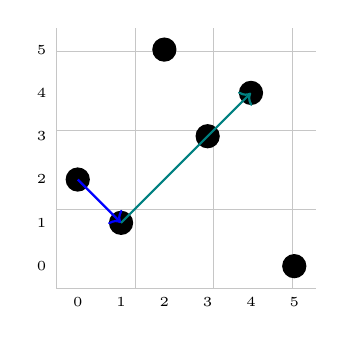
\begin{tikzpicture}[x=0.55cm,y=0.55cm]
\draw[gray!45,very thin] (0,0) grid (6,6);
\fill[black] (0.5,2.5) circle (0.28);
\fill[black] (1.5,1.5) circle (0.28);
\fill[black] (2.5,5.5) circle (0.28);
\fill[black] (3.5,3.5) circle (0.28);
\fill[black] (4.5,4.5) circle (0.28);
\fill[black] (5.5,0.5) circle (0.28);
\draw[->,thick,blue] (0.5,2.5) -- (1.5,1.5);
\draw[->,thick,teal] (1.5,1.5) -- (4.5,4.5);
\node[font=\tiny,below] at (0.5,0) {0};
\node[font=\tiny,left] at (0,0.5) {0};
\node[font=\tiny,below] at (1.5,0) {1};
\node[font=\tiny,left] at (0,1.5) {1};
\node[font=\tiny,below] at (2.5,0) {2};
\node[font=\tiny,left] at (0,2.5) {2};
\node[font=\tiny,below] at (3.5,0) {3};
\node[font=\tiny,left] at (0,3.5) {3};
\node[font=\tiny,below] at (4.5,0) {4};
\node[font=\tiny,left] at (0,4.5) {4};
\node[font=\tiny,below] at (5.5,0) {5};
\node[font=\tiny,left] at (0,5.5) {5};
\end{tikzpicture}
\par\small (a) $\pi=(2,1,5,3,4,0)$, a Costas array
\end{minipage}\hfill
\begin{minipage}{0.47\linewidth}\centering
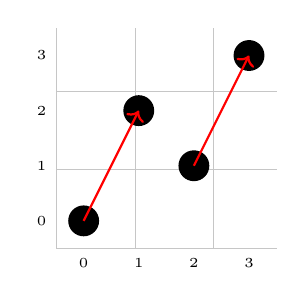
\begin{tikzpicture}[x=0.7cm,y=0.7cm]
\draw[gray!45,very thin] (0,0) grid (4,4);
\fill[black] (0.5,0.5) circle (0.28);
\fill[black] (1.5,2.5) circle (0.28);
\fill[black] (2.5,1.5) circle (0.28);
\fill[black] (3.5,3.5) circle (0.28);
\draw[->,thick,red] (0.5,0.5) -- (1.5,2.5);
\draw[->,thick,red] (2.5,1.5) -- (3.5,3.5);
\node[font=\tiny,below] at (0.5,0) {0};
\node[font=\tiny,left] at (0,0.5) {0};
\node[font=\tiny,below] at (1.5,0) {1};
\node[font=\tiny,left] at (0,1.5) {1};
\node[font=\tiny,below] at (2.5,0) {2};
\node[font=\tiny,left] at (0,2.5) {2};
\node[font=\tiny,below] at (3.5,0) {3};
\node[font=\tiny,left] at (0,3.5) {3};
\end{tikzpicture}
\par\small (b) $\pi=(0,2,1,3)$, not Costas
\end{minipage}
\caption{(a) An order-6 Costas array. The two arrows shown, $(1,-1)$ and $(3,3)$, are two of
its 15 displacements, and all 15 differ. (b) A permutation that fails: the arrows from column
0 to column 1 and from column 2 to column 3 are both $(1,2)$. Dots are at $(i,\pi(i))$ with
row 0 at the bottom.}
\label{fig:primer}
\end{figure}

\subsection{Checking the condition lag by lag}

It is convenient to group the displacements by their horizontal component, the \emph{lag}
$s=j-i$. For each lag $s$ the condition says that the vertical differences
$\pi(x+s)-\pi(x)$, for $x=0,\dots,n-1-s$, are all different. Writing these rows out gives
the \emph{difference triangle} of $\pi$. For Figure~\ref{fig:primer}(a):
\begin{center}
\begin{tabular}{@{}r l@{}}
lag 1: & $-1,\ \ 4,\ -2,\ \ 1,\ -4$\\
lag 2: & $\ \ 3,\ \ 2,\ -1,\ -3$\\
lag 3: & $\ \ 1,\ \ 3,\ -5$\\
lag 4: & $\ \ 2,\ -1$\\
lag 5: & $-2$
\end{tabular}
\end{center}
Every row has distinct entries, so the array is Costas. (Entries may repeat \emph{between}
rows, since those arrows have different horizontal components.)

\subsection{What is known}

Costas arrays were introduced in the 1960s for sonar and radar: a frequency-hopping signal
whose hop pattern is a Costas array has an ideal ``thumbtack'' ambiguity function, since no
shift in time and frequency makes more than one hop coincide~\cite{costas1984}. Two algebraic
constructions produce infinite families~\cite{golombtaylor1984}:
\begin{itemize}
\item \emph{Welch}: for a prime $p$ and a primitive root $g$ modulo $p$,
$\pi(i)=g^{\,i+1}\bmod p\;-\;1$ for $i=0,\dots,p-2$ is a Costas array of order $p-1$. With
$p=7$ and $g=3$ this gives exactly Figure~\ref{fig:primer}(a).
\item \emph{Lempel--Golomb}: from primitive elements of the finite field of $q$ elements, an
array of order $q-2$; variants give $q-3$ and a few others.
\end{itemize}
Every order up to 31 is reached by a construction or by search, and all Costas arrays have
been enumerated exhaustively up to order 29~\cite{drakakis2011}. Orders 32 and 33 are the
smallest with no known example~\cite{drakakis2006}. Neither construction reaches them, and
exhaustive search is far beyond reach: there are $32!\approx2.6\times10^{35}$ permutations,
and the cost of exhaustive enumeration grows rapidly with the order.

%======================================================================
\section{Symmetry, and the transpose-symmetric subclass}\label{sec:symmetry}
This section explains why transpose symmetry is the natural subclass to study, being the only symmetry of the square that a Costas array can have, and what its members look like. It separates what is known from the literature from what was computed in this project.

%======================================================================

\subsection{The symmetries of the square}

Rotating the grid by a multiple of $90^\circ$, or reflecting it in a horizontal, vertical or
diagonal line, maps permutation matrices to permutation matrices. These eight motions form
the dihedral group $D_4$. Each of them maps Costas arrays to Costas arrays, because it maps
the set of displacement vectors one-to-one onto another set of vectors. So Costas arrays come
in families of up to eight. An array is \emph{geometrically symmetric} if some non-identity motion maps it
to itself.

The following classification is elementary background, and we make no claim to its novelty.
Taylor, Rickard and Drakakis enumerate diagonal symmetry alongside symmetry types that are not
motions of the square~\cite{taylor2009}; the classification below explains why, among the motions,
diagonal symmetry is the only one that needs enumerating. We include a short proof because it fixes the scope of the present search, and to keep
the report self-contained.

\begin{proposition}[Only transpose symmetry is possible]\label{prop:onlytranspose}
For $n\ge3$, the only non-identity motions that can fix a Costas array are the reflections in
the two diagonals.
\end{proposition}
\begin{proof}
A reflection in the vertical axis fixes $\pi$ only if $\pi(i)=\pi(n-1-i)$ for every $i$. For any
$i\ne n-1-i$ that puts two dots in one row, which is impossible for a permutation. A reflection in
the horizontal axis requires $\pi(i)=n-1-\pi(i)$ for every $i$, putting every dot in the same
central row, which is also impossible.

For the $180^\circ$ rotation, invariance gives $\pi(n-1-i)=n-1-\pi(i)$ for every $i$. Take
columns $i<j$, and their rotated pair $n-1-j<n-1-i$. The two pairs have the same displacement:
\[
\begin{aligned}
(n-1-i)-(n-1-j) &= j-i,\\
\pi(n-1-i)-\pi(n-1-j) &= \bigl(n-1-\pi(i)\bigr)-\bigl(n-1-\pi(j)\bigr)=\pi(j)-\pi(i).
\end{aligned}
\]
The two pairs of columns coincide only when $i+j=n-1$. For $n\ge3$, the pair $i=0$, $j=1$ has
$i+j=1\ne n-1$, so two distinct pairs of dots have the same displacement, contradicting the Costas
condition. Rotations by $90^\circ$ and $270^\circ$ square to the $180^\circ$ rotation, so they are
excluded too. That leaves the two diagonal reflections, which are conjugate under the group.
\end{proof}

Reflection in the main diagonal swaps the roles of rows and columns: it maps $\pi$ to
$\pi^{-1}$. So an array is transpose-symmetric exactly when $\pi=\pi^{-1}$, i.e.\ when
$\pi$ is an involution. By the proposition, studying involutions covers every geometrically symmetric
Costas array, since the other diagonal is conjugate to it.

\subsection{What a transpose-symmetric array looks like}

An involution consists of fixed points, coordinates $c$ with $\pi(c)=c$ whose dots lie
on the main diagonal, and transpositions $(a\,b)$ with $\pi(a)=b$, $\pi(b)=a$, whose
two dots are mirror images across the diagonal. Figure~\ref{fig:sym} shows two real examples.

\begin{figure}[H]
\centering
\begin{minipage}{0.5\linewidth}\centering
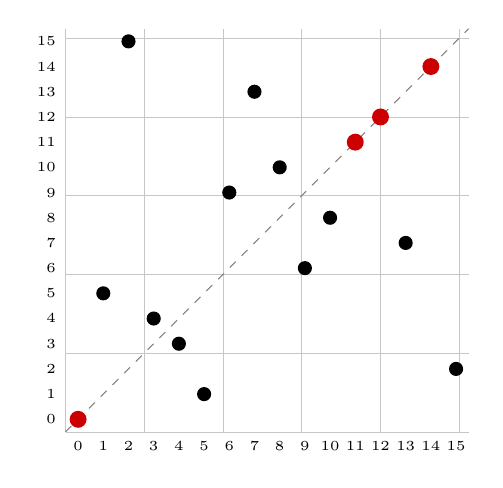
\begin{tikzpicture}[x=0.32cm,y=0.32cm]
\draw[gray!45,very thin] (0,0) grid (16,16);
\draw[gray,dashed] (0,0) -- (16,16);
\fill[red!80!black] (0.5,0.5) circle (0.336);
\fill[black] (1.5,5.5) circle (0.28);
\fill[black] (2.5,15.5) circle (0.28);
\fill[black] (3.5,4.5) circle (0.28);
\fill[black] (4.5,3.5) circle (0.28);
\fill[black] (5.5,1.5) circle (0.28);
\fill[black] (6.5,9.5) circle (0.28);
\fill[black] (7.5,13.5) circle (0.28);
\fill[black] (8.5,10.5) circle (0.28);
\fill[black] (9.5,6.5) circle (0.28);
\fill[black] (10.5,8.5) circle (0.28);
\fill[red!80!black] (11.5,11.5) circle (0.336);
\fill[red!80!black] (12.5,12.5) circle (0.336);
\fill[black] (13.5,7.5) circle (0.28);
\fill[red!80!black] (14.5,14.5) circle (0.336);
\fill[black] (15.5,2.5) circle (0.28);
\node[font=\tiny,below] at (0.5,0) {0};
\node[font=\tiny,left] at (0,0.5) {0};
\node[font=\tiny,below] at (1.5,0) {1};
\node[font=\tiny,left] at (0,1.5) {1};
\node[font=\tiny,below] at (2.5,0) {2};
\node[font=\tiny,left] at (0,2.5) {2};
\node[font=\tiny,below] at (3.5,0) {3};
\node[font=\tiny,left] at (0,3.5) {3};
\node[font=\tiny,below] at (4.5,0) {4};
\node[font=\tiny,left] at (0,4.5) {4};
\node[font=\tiny,below] at (5.5,0) {5};
\node[font=\tiny,left] at (0,5.5) {5};
\node[font=\tiny,below] at (6.5,0) {6};
\node[font=\tiny,left] at (0,6.5) {6};
\node[font=\tiny,below] at (7.5,0) {7};
\node[font=\tiny,left] at (0,7.5) {7};
\node[font=\tiny,below] at (8.5,0) {8};
\node[font=\tiny,left] at (0,8.5) {8};
\node[font=\tiny,below] at (9.5,0) {9};
\node[font=\tiny,left] at (0,9.5) {9};
\node[font=\tiny,below] at (10.5,0) {10};
\node[font=\tiny,left] at (0,10.5) {10};
\node[font=\tiny,below] at (11.5,0) {11};
\node[font=\tiny,left] at (0,11.5) {11};
\node[font=\tiny,below] at (12.5,0) {12};
\node[font=\tiny,left] at (0,12.5) {12};
\node[font=\tiny,below] at (13.5,0) {13};
\node[font=\tiny,left] at (0,13.5) {13};
\node[font=\tiny,below] at (14.5,0) {14};
\node[font=\tiny,left] at (0,14.5) {14};
\node[font=\tiny,below] at (15.5,0) {15};
\node[font=\tiny,left] at (0,15.5) {15};
\end{tikzpicture}
\par\small (a) order 16, fixed points $\{0,11,12,14\}$
\end{minipage}\hfill
\begin{minipage}{0.46\linewidth}\centering
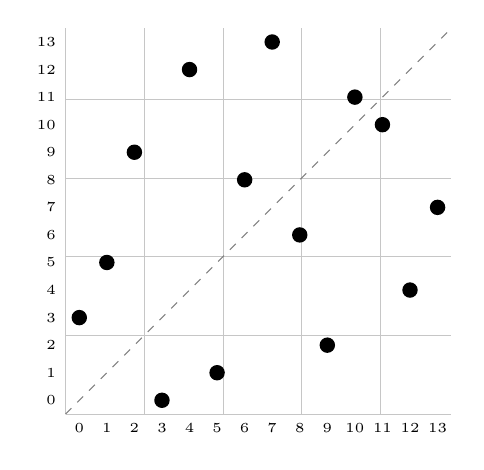
\begin{tikzpicture}[x=0.35cm,y=0.35cm]
\draw[gray!45,very thin] (0,0) grid (14,14);
\draw[gray,dashed] (0,0) -- (14,14);
\fill[black] (0.5,3.5) circle (0.28);
\fill[black] (1.5,5.5) circle (0.28);
\fill[black] (2.5,9.5) circle (0.28);
\fill[black] (3.5,0.5) circle (0.28);
\fill[black] (4.5,12.5) circle (0.28);
\fill[black] (5.5,1.5) circle (0.28);
\fill[black] (6.5,8.5) circle (0.28);
\fill[black] (7.5,13.5) circle (0.28);
\fill[black] (8.5,6.5) circle (0.28);
\fill[black] (9.5,2.5) circle (0.28);
\fill[black] (10.5,11.5) circle (0.28);
\fill[black] (11.5,10.5) circle (0.28);
\fill[black] (12.5,4.5) circle (0.28);
\fill[black] (13.5,7.5) circle (0.28);
\node[font=\tiny,below] at (0.5,0) {0};
\node[font=\tiny,left] at (0,0.5) {0};
\node[font=\tiny,below] at (1.5,0) {1};
\node[font=\tiny,left] at (0,1.5) {1};
\node[font=\tiny,below] at (2.5,0) {2};
\node[font=\tiny,left] at (0,2.5) {2};
\node[font=\tiny,below] at (3.5,0) {3};
\node[font=\tiny,left] at (0,3.5) {3};
\node[font=\tiny,below] at (4.5,0) {4};
\node[font=\tiny,left] at (0,4.5) {4};
\node[font=\tiny,below] at (5.5,0) {5};
\node[font=\tiny,left] at (0,5.5) {5};
\node[font=\tiny,below] at (6.5,0) {6};
\node[font=\tiny,left] at (0,6.5) {6};
\node[font=\tiny,below] at (7.5,0) {7};
\node[font=\tiny,left] at (0,7.5) {7};
\node[font=\tiny,below] at (8.5,0) {8};
\node[font=\tiny,left] at (0,8.5) {8};
\node[font=\tiny,below] at (9.5,0) {9};
\node[font=\tiny,left] at (0,9.5) {9};
\node[font=\tiny,below] at (10.5,0) {10};
\node[font=\tiny,left] at (0,10.5) {10};
\node[font=\tiny,below] at (11.5,0) {11};
\node[font=\tiny,left] at (0,11.5) {11};
\node[font=\tiny,below] at (12.5,0) {12};
\node[font=\tiny,left] at (0,12.5) {12};
\node[font=\tiny,below] at (13.5,0) {13};
\node[font=\tiny,left] at (0,13.5) {13};
\end{tikzpicture}
\par\small (b) order 14, no fixed points
\end{minipage}
\caption{Two transpose-symmetric Costas arrays. Fixed points are red, on the dashed diagonal;
every other dot has its mirror image across the diagonal. In (a) the fixed points have
pairwise distances 1, 2, 3, 11, 12 and 14, all different, which Lemma~\ref{lem:golombprimer}
says must happen.}
\label{fig:sym}
\end{figure}

\begin{lemma}[Fixed points form a Golomb ruler]\label{lem:golombprimer}
In a transpose-symmetric Costas array, the pairwise differences between fixed points are all
distinct.
\end{lemma}
\begin{proof}
Fixed points $a<b$ have dots $(a,a)$ and $(b,b)$, with displacement $(b-a,b-a)$. Two pairs of
fixed points at the same distance would give the same displacement.
\end{proof}

A set of integers with all pairwise differences distinct is a Golomb ruler. Short
Golomb rulers with many marks are impossible: the shortest ruler with 8 marks has length 34, a known value in the literature on Golomb
rulers that Proposition~\ref{prop:f} confirms independently by exhaustive search,
more than the 31 available on a $32\times32$ board. Since the number $f$ of fixed points has
the same parity as $n$, at order 32
\[
f\in\{0,2,4,6\}.
\]

\subsection{Constructions in the literature}
Some algebraic constructions in the literature produce symmetric arrays directly. The Lempel
construction, the special case of the Lempel--Golomb construction in which the two primitive
elements coincide, sets $\pi(i)=j$ exactly when $\alpha^i+\alpha^j=1$ in the field of $q$
elements. That relation is symmetric in $i$ and $j$, so every Lempel array is
transpose-symmetric. It has order $q-2$ for each prime power $q$~\cite{golombtaylor1984}.
Drakakis, Gow and O'Carroll identify a second symmetric subfamily of the Lempel--Golomb
construction: when $q=r^2$ is a square, the arrays with $\beta=\alpha^r$~\cite{dgo2006}. Both
families have order $q-2$. Order 32 would require $q=34$, which is not a prime power, so neither
family, and no other known construction, gives a symmetric array of order 32.

\subsection{Enumerations of symmetric arrays in the literature}\label{sec:censuses}
Transpose-symmetric arrays are called \emph{diagonal} in the literature. Their numbers have been
determined by exhaustive search twice.
\begin{itemize}
\item Brown, Cenki, Games, Rushanan, Moreno and Pei tabulated the numbers of diagonal,
anti-reflective and consecutive Costas arrays of each order up to 32~\cite{brown1993}.
\item Taylor, Rickard and Drakakis recomputed these counts~\cite{taylor2009}. Their exhaustive
search is a backtracking search over permutations, using a midpoint test for the Costas condition
(the Ladendorf method) and symmetry reduction. For orders up to 27 they also tested every array in
the database of all known Costas arrays: the paper's text says the counts for those orders were
obtained that way, and its table caption says they were cross-checked that way. Above order 27,
including order 32, the counts come from the exhaustive search alone. They corrected a few entries
of the 1993 table, extended it to order 36 and to further symmetry types, and identified which
arrays are sporadic.
They found no sporadic symmetric array at any order from 24 to 36.
\end{itemize}
Both tables record zero diagonal Costas arrays of order 32. In the 2009 table that entry is
marked as previously known, so it is a 1993 result confirmed in 2009. The non-existence of a
transpose-symmetric Costas array of order 32 has therefore been in the literature since 1993, and
it is independently confirmed by the search reported here, which shares neither method nor
software with either enumeration.

The 2009 table counts \emph{unique} arrays, one per equivalence family under the motions of the
square. Each family of diagonal arrays contains exactly two transpose-symmetric arrays: an array
and its $180^\circ$ rotation, which differ by Proposition~\ref{prop:onlytranspose}. So its counts
should be exactly half of counts of individual arrays, which is what Table~\ref{tab:symcounts}
compares.

\subsection{How rare they are}

In this project, transpose-symmetric Costas arrays were enumerated exhaustively up to order 24
by three independent implementations of an involution search, which agree on the size of the
search tree. The counts in Table~\ref{tab:symcounts} come from those searches, not from the
literature. At every order in the table they are exactly twice the 2009 class counts, as the
counting conventions require, and both give zero at order 24. The 158 arrays of orders 12--22
are used throughout this project as test data.

\begin{table}[H]
\centering
\begin{tabular}{@{}rrrrrr@{}}
\toprule
order & $f=0$ & $f=2$ & $f=4$ & total & classes in~\cite{taylor2009} \\
\midrule
12 & 2 & 28 & 4 & 34 & 17 \\
14 & 4 & 30 & 12 & 46 & 23 \\
16 & 4 & 28 & 8 & 40 & 20 \\
18 & 0 & 14 & 6 & 20 & 10 \\
20 & 0 & 6 & 2 & 8 & 4 \\
22 & 0 & 8 & 2 & 10 & 5 \\
24 & & & & 0 & 0 \\
\bottomrule
\end{tabular}
\caption{Transpose-symmetric Costas arrays by order and number of fixed points, from this
project's exhaustive searches, with the number of equivalence classes of diagonal arrays reported
in~\cite{taylor2009}. Every count is exactly twice the class count. None has
six fixed points, and there are none at all at order 24. A direct search at order 32, run to completion,
visits $1.355\times10^{11}$ nodes (Section~\ref{sec:direct}).}
\label{tab:symcounts}
\end{table}

%======================================================================
\section{Earlier structural results in this project}\label{sec:earlier}
This section summarises structural results obtained earlier in this project, before the campaign reported here. They motivate the change of decomposition adopted in Part~II, and they provide independent checks on its outcome.

%======================================================================

Before this campaign, the project attacked the order-32 symmetric problem through the
geometry of long displacements. This section records those results, which the present
search extends and with which it is consistent.

\paragraph{Large-large pairs.} Call a pair of coordinates $\{x,y\}$ large-large if
both $|x-y|\ge16$ and $|\pi(x)-\pi(y)|\ge16$: the two dots are far apart both horizontally and
vertically. Let $Z(\pi)$ be the number of large-large pairs. For an involution $\pi$ the map
$\tau\{x,y\}=\{\pi(x),\pi(y)\}$ permutes large-large pairs, and since $\pi^2=\mathrm{id}$ its
orbits have size 1 or 2. A pair is fixed by $\tau$ exactly when both points are fixed points,
or when $\{x,y\}$ is itself a transposition. This gives the \emph{orbit decomposition}
\[
Z = I_F + q + 2C,
\]
where $I_F$ counts large-large pairs of fixed points, $q$ the transpositions of length at
least 16, and $C$ the orbits of size two. It was verified on 12{,}000 random involutions and
on all 158 arrays of Table~\ref{tab:symcounts}.

\paragraph{$Z=0$ is impossible.} Sort the displacements into four ``quadrants'' by whether
their horizontal and vertical components are short ($<16$) or long. A counting identity shows
that the short-short quadrant cannot be empty at order 32, and an automorphism argument shows
that the two mixed quadrants cannot both be empty. So the large-large quadrant is the only one
that could be empty, and that is the case $Z=0$. It forces all transposition lengths and all
fixed-point separations below 16, and hence $f\in\{2,4\}$. Both cases were closed by
exhaustive structural search: for $f=2$ by the chain $32{,}769{,}242\to9{,}180\to4\to0$
candidates under successively stronger sieves, and for $f=4$ by
$2{,}735\to20{,}360\to20{,}360\to0$.

\paragraph{$Z=1$ is impossible.} With $Z=1$ there is exactly one large-large pair: either a
single long transposition (branch T) or a single long pair of fixed points (branch F). That
yields seven labels by branch and $f$, all closed.

\begin{table}[H]
\centering
\begin{tabular}{@{}llll@{}}
\toprule
branch & $f$ & certificate & method \\
\midrule
T & 0 & $36\to1\to0$ & one residue, eliminated by the Costas condition \\
F & 2 & $36\to0$ & structural \\
T & 2 & $72\to0$ & full Costas search \\
T & 6 & --- & deductive: no 6-mark ruler fits a window of 15 \\
F & 6 & $728\to0$ & structural and full Costas \\
F & 4 & $19{,}405\to0$ & structural and full Costas \\
T & 4 & $2{,}735\to0$ & full Costas search \\
\bottomrule
\end{tabular}
\caption{The seven $Z=1$ labels and their closures. Each count is the number of root
configurations searched, every one ending in a fail-closed terminal status.}
\label{tab:z1}
\end{table}

\paragraph{Why a different decomposition.} After these results, every remaining candidate
had $Z\ge2$. The next layer, $Z=2$, splits by the orbit decomposition into two structural
types and ten feasible cells, each needing its own bespoke search, and the layers grow
quickly from there. The present campaign takes a different route. It partitions by the
\emph{fixed-point set} rather than by $Z$, and hands each region to general SAT
technology, with a decomposition designed around the fixed points. Two consistency checks link
the two programmes:
\begin{itemize}
\item the $Z=2$ analysis derived, independently, a catalogue of reflection-canonical
fixed-point sets with totals 1, 256, 13{,}587 and 31{,}103 for $f=0,2,4,6$, exactly the region
counts of Section~\ref{sec:framework};
\item every candidate excluded by the $Z=0$ and $Z=1$ theorems lies in some region, and all
regions are now closed, so the two programmes agree.
\end{itemize}
The earlier results are finite computations with fail-closed status, not formally certified,
like the present ones.

\part{Method}

\section{The fixed-point partition}\label{sec:framework}
This section turns the Golomb-ruler property into an exhaustive partition of the order-32 problem. It gives the formal definitions used in the rest of the report and derives the 44{,}947 regions.

%======================================================================

Throughout, $n=32$ and coordinates are $[n]=\{0,\dots,31\}$, starting at zero.

\paragraph{Geometric convention.} The dot of column $i$ is at $(i,\pi(i))$: the first
coordinate is the column, the second the row. For two columns $i<j$ the displacement is
$(j-i,\ \pi(j)-\pi(i))$, whose first component, the lag $s=j-i$, is positive.
Distinctness of all displacements is therefore the same as requiring, for each lag
$s=1,\dots,31$ separately, that the vertical differences $\pi(x+s)-\pi(x)$ over
$x=0,\dots,31-s$ be pairwise distinct. The SAT encoding uses exactly this lag-by-lag form.

\begin{definition}
A permutation $\pi$ of $[n]$ is \emph{Costas} if the vectors $(j-i,\pi(j)-\pi(i))$,
$0\le i<j\le 31$, are pairwise distinct; it is a \emph{Costas involution} if also
$\pi^2=\mathrm{id}$. Its fixed-point set is $\Fix(\pi)=\{i:\pi(i)=i\}$, with $f=|\Fix(\pi)|$.
\end{definition}

\begin{example}[A collision]
If $\pi(i+s)-\pi(i)=\delta=\pi(j+s)-\pi(j)$ for some $i\ne j$, the column pairs $(i,i+s)$
and $(j,j+s)$ both have displacement $(s,\delta)$, and $\pi$ is not Costas. In the encoding
of Section~\ref{sec:encoding}, the indicators $p_{s,i,\delta}$ and $p_{s,j,\delta}$ are then
both forced true, violating the at-most-one constraint for $(s,\delta)$.
\end{example}

\begin{lemma}\label{lem:sym}
The permutation matrix of $\pi$ is transpose-symmetric if and only if $\pi$ is an involution.
\end{lemma}
\begin{proof}
The matrix has dots $(i,\pi(i))$; its transpose has dots $(\pi(i),i)$, which form the matrix
of $\pi^{-1}$. They coincide iff $\pi=\pi^{-1}$.
\end{proof}

An involution splits $[n]$ into fixed points and disjoint transpositions $(a\,b)$ with
$\pi(a)=b$, $\pi(b)=a$. Since $n$ is even, $f$ is even.

\begin{lemma}[Fixed points form a Golomb ruler]\label{lem:golomb}
If $\pi$ is a Costas involution, the pairwise differences of $\Fix(\pi)$ are distinct.
\end{lemma}
\begin{proof}
For fixed points $a<b$ the dots $(a,a)$ and $(b,b)$ have displacement $(b-a,b-a)$. Two
different pairs with the same difference would repeat a displacement.
\end{proof}

\begin{proposition}\label{prop:f}
At order 32, $f\in\{0,2,4,6\}$.
\end{proposition}
\begin{proof}
$f$ is even. An exhaustive backtracking search over 8-element subsets of $[32]$ with
distinct pairwise differences finds none (Algorithm~\ref{alg:enum}, run to completion), so
there is no Golomb ruler with 8 or more marks in $[32]$, since any such ruler contains an
8-mark one. This agrees with the known optimal 8-mark length, 34. Hence $f\le 6$.
\end{proof}

\begin{lemma}[Reflection]\label{lem:refl}
Let $\rho(i)=31-i$. If $\pi$ is a Costas involution, so is $\rho\pi\rho$, and
$\Fix(\rho\pi\rho)=\rho(\Fix\pi)$.
\end{lemma}
\begin{proof}
$(\rho\pi\rho)^2=\rho\pi^2\rho=\mathrm{id}$. The array of $\rho\pi\rho$ is that of $\pi$
rotated by $180^\circ$, which negates every displacement and so preserves distinctness.
Finally $\rho\pi\rho(i)=i\iff\pi(\rho(i))=\rho(i)$.
\end{proof}

\begin{definition}[Region]
For a Golomb ruler $F\subseteq[n]$ with $|F|\in\{0,2,4,6\}$, the region $R_F$ is the set of
Costas involutions $\pi$ with $\Fix(\pi)=F$ exactly. $F$ is reflection-canonical if,
as a sorted tuple, $F\le\rho(F)$ lexicographically. Regions are named \code{R00000},
\code{R00001}, \dots{} in the order of Algorithm~\ref{alg:enum}; for a named region,
$F(\code{R}\ldots)$ denotes its fixed-point set.
\end{definition}

\begin{theorem}[Partition]\label{thm:partition}
Every Costas involution of order 32 lies in exactly one region and, after applying $\rho$ if
necessary, in a reflection-canonical one. Hence a transpose-symmetric Costas array of order
32 exists iff some reflection-canonical region is non-empty.
\end{theorem}
\begin{proof}
$\Fix(\pi)$ is unique, a Golomb ruler (Lemma~\ref{lem:golomb}), and of admissible size
(Proposition~\ref{prop:f}); Lemma~\ref{lem:refl} maps a non-canonical case to the canonical
region of $\rho(F)$.
\end{proof}

\begin{figure}[H]
\centering
\begin{minipage}{0.9\linewidth}
\small
Algorithm 1 (region enumeration, \code{regions.py})\label{alg:enum}
\begin{enumerate}[nosep, label=\arabic*.]
\item emit the empty set as \code{R00000};
\item for $f=2,4,6$, and for each $f$-subset $F$ of $[32]$ in lexicographic order:
\item \quad reject $F$ unless its $\binom{f}{2}$ positive differences are distinct;
\item \quad reject $F$ unless $F\le\rho(F)$ as sorted tuples;
\item \quad emit $F$ with the next region number, its size, diameter $\max F-\min F$, and
its number of even elements.
\end{enumerate}
For the 8-mark check of Proposition~\ref{prop:f} the same distinct-difference test is applied
by backtracking from mark 0 with span at most 31; it returns no ruler.
\end{minipage}
\end{figure}

\begin{table}[H]
\centering
\begin{tabular}{@{}rrrr@{}}
\toprule
$f$ & Golomb rulers in $[32]$ & fixed by $\rho$ & canonical regions \\
\midrule
0 & 1 & 1 & 1 \\
2 & 496 & 16 & 256 \\
4 & 27{,}174 & 0 & 13{,}587 \\
6 & 62{,}206 & 0 & 31{,}103 \\
\midrule
total & 89{,}877 & 17 & 44{,}947 \\
\bottomrule
\end{tabular}
\caption{Region counts. Canonical $=(\text{raw}+\text{fixed})/2$. A $\rho$-fixed set with
four or more marks contains $a<b$ and $31-b<31-a$, which repeat the difference $b-a$, so
none is a Golomb ruler. Script and output digests are in Appendix~\ref{app:digests}.}
\label{tab:regions}
\end{table}

\begin{definition}[Seed refutation]\label{def:seed}
For free $x<y$, form the multiset of displacement vectors between every pair of dots in
$\{(c,c):c\in F\}\cup\{(x,y),(y,x)\}$, each pair taken in column order. The pair $\{x,y\}$ is
\emph{seed-refuted} for $F$ if this multiset contains a repeated vector.
\end{definition}

\begin{lemma}\label{lem:seed}
If $\{x,y\}$ is seed-refuted, no member of $R_F$ contains the transposition $(x\,y)$, and the
encoding of Section~\ref{sec:encoding} refutes $x_{xy}$ by unit propagation alone.
\end{lemma}
\begin{proof}
Any such $\pi$ contains all of those dots. In the encoding, $x_{xy}$ forces $h_{xy},h_{yx}$
(clause family 1), which together with the constant fixed-point values force two
displacement indicators with the same $(s,\delta)$ true (family 5), and their binary
at-most-one clause (family 6) is then falsified.
\end{proof}

%======================================================================
\section{SAT encoding of a region}\label{sec:encoding}
This section gives the propositional encoding of a single region, proves it exact, and records how it was validated. Every solver verdict in the report rests on this encoding.

%======================================================================

\paragraph{Notation.} For literals $q_1,\dots,q_m$:
$\ALO(q_1,\dots,q_m)=(q_1\vee\dots\vee q_m)$,
$\AMO(q_1,\dots,q_m)=\bigwedge_{1\le i<j\le m}(\neg q_i\vee\neg q_j)$ (pairwise), and
$\EO=\ALO\wedge\AMO$.

Fix a region $F$ and let $V=[n]\setminus F$.

\paragraph{Variables.}
\begin{itemize}
\item $x_{ab}$ for $a,b\in V$, $a<b$: transposition $(a\,b)$ present.
\item $h_{ij}$ for $i,j\in V$, $i\ne j$: $\pi(i)=j$.
\item $p_{s,x,\delta}$ for $1\le s\le 31$, $0\le x\le 31-s$, $-31\le\delta\le 31$, created only
when \emph{realisable}: there are permitted values $u$ for column $x$ and $w$ for column $x+s$
with $w-u=\delta$. A fixed column $c\in F$ permits only $u=c$; a free column permits every
$u\in V$ other than itself.
\end{itemize}
The literal $[\pi(i)=j]$ means $h_{ij}$ for $i,j\in V$; it is the constant \emph{true} if
$i=j\in F$, and \emph{false} if exactly one of $i,j$ is in $F$.

\paragraph{Clauses.}
\begin{enumerate}
\item \emph{Edge--map link:} $(\neg x_{ab}\vee h_{ab})$, $(\neg x_{ab}\vee h_{ba})$,
$(\neg h_{ab}\vee x_{ab})$ for $a<b$.
\item \emph{One image per free coordinate:} $\EO(\{h_{ij}\}_{j\in V\setminus\{i\}})$ for
each $i\in V$.
\item \emph{One transposition per free coordinate:} $\EO(\{x_e: c\in e\})$ for each $c\in V$.
\item \emph{Distinct transposition lengths:} $\AMO(\{x_{a,a+d}\})$ for each length $d$.
\item \emph{Displacement indicators:} for each column pair $(x,x+s)$ and permitted values
$(u,w)$, the clause $\neg[\pi(x)=u]\vee\neg[\pi(x+s)=w]\vee p_{s,x,w-u}$, with constant-true
literals removed. There are three cases: both columns free (a three-literal clause); one
column fixed (a two-literal clause); both fixed (the unit clause $p_{s,x,w-u}$, so
fixed-to-fixed displacements are asserted outright and can collide with displacements of
transpositions).
\item \emph{Costas:} $\AMO(\{p_{s,x,\delta}\}_x)$ for each $(s,\delta)$.
\end{enumerate}

\begin{remark}
Given family (1), families (2) and (3) imply each other: an image $h_{ij}$ forces the edge
$x_{ij}$, and an edge forces both images. Both are kept because they propagate differently,
through the map and through the matching. Family (4) is implied by the Costas property,
since a transposition of length $d$ has internal displacement $(d,-d)$, and is kept for
propagation. The proof of Theorem~\ref{thm:exact} uses (1), (3), (5) and (6).
\end{remark}

\begin{theorem}[Exactness]\label{thm:exact}
The set of edge-variable projections of the models of the encoding is in bijection with the
set of Costas involutions $\pi$ with $\Fix(\pi)=F$.
\end{theorem}
\begin{proof}
Let $\alpha$ be a model. By (3) its true edges form a perfect matching of $V$; with $F$ fixed,
this defines an involution $\pi$ with $\Fix(\pi)=F$ exactly, because no variable expresses
$\pi(i)=i$ for $i\in V$ and (3) places every $i\in V$ in a transposition. By (1) and (2), the
$h$-variables agree with $\pi$. By (5), every displacement that $\pi$ realises has its
indicator true, so (6) forbids two column pairs at one lag with the same vertical difference:
$\pi$ is Costas. Conversely, a Costas involution with fixed set $F$, with $p$ set to true
exactly on realised displacements, satisfies every clause. The map from projections to
involutions is injective, since the projection is the matching itself. Indicators for
displacements that are not realised are not forced false, so several models can share one
projection; the bijection is therefore stated for projections.
\end{proof}

\begin{remark}[Enumeration blocks edge projections]\label{rem:projblock}
The theorem is a bijection between involutions and edge-variable projections, not between
involutions and complete assignments. Any validation by model enumeration must therefore block the
edge projection, not the complete Boolean model: at order 10, a single edge projection has at least
64 complete models that differ only in unrealised indicators.
\end{remark}

\begin{table}[H]
\centering
\begin{tabular}{@{}rrrrrrr@{}}
\toprule
$f$ & $|V|$ & edge vars & map vars & indicator vars & total vars & clauses \\
\midrule
0 & 32 & 496 & 992 & 31{,}185 & 32{,}673 & 824{,}506 \\
2 & 30 & 435 & 870 & 29{,}030--29{,}087 & 30{,}335--30{,}392 & 666{,}858--669{,}798 \\
4 & 28 & 378 & 756 & 25{,}277--26{,}789 & 26{,}411--27{,}923 & 527{,}716--533{,}367 \\
6 & 26 & 325 & 650 & 22{,}943--24{,}290 & 23{,}918--25{,}265 & 412{,}138--418{,}785 \\
\bottomrule
\end{tabular}
\caption{Formula sizes. Edge and map counts are $\binom{|V|}{2}$ and $|V|(|V|-1)$ for every
region; indicator and clause counts depend on $F$ and are given as ranges over five sampled
regions per class (the $f=0$ class has one region).}
\label{tab:sizes}
\end{table}

\paragraph{Validation.}
\begin{itemize}
\item \emph{Exhaustive equivalence at orders 8 and 10.} For each of the 39 and 106 fixed-point
sets, the comparison is made at the level of edge projections, not complete assignments
(Remark~\ref{rem:projblock}). After each model $\alpha$ the enumerator adds the
projection-blocking clause
\[
\bigvee_{\alpha(x_{ab})=1}\neg x_{ab}\;\vee\bigvee_{\alpha(x_{ab})=0}x_{ab},
\]
over all edge variables of the region, so each matching is returned once, however its indicators
are completed. Each decoded involution is checked independently for being a permutation and an
involution, for its exact fixed-point set and for distinct displacements, and any duplicate is
rejected outside the solver. Conversely, every Costas involution found by brute-force enumeration of
the region's perfect matchings is checked to satisfy every clause under its canonical assignment, in
which each indicator is true exactly when its displacement is realised. The first direction places
the projected set inside the direct set, and the second places the direct set inside the projected
set; comparing the sorted sets confirms that they are equal in every region
(Table~\ref{tab:projval}).
\item \emph{Regression.} All 158 known transpose-symmetric Costas arrays of orders 12--22
satisfy their region's CNF under direct clause evaluation.
\item \emph{Determinism.} All 225 Stage-1 CNFs (Section~\ref{sec:campaign}) were regenerated
on the cluster and matched their recorded SHA-256 digests byte for byte.
\end{itemize}

\begin{table}[H]
\centering
\small
\begin{tabular}{@{}rrrrrcl@{}}
\toprule
order & regions & solver calls & projected & direct & failures & set digest \\
\midrule
8 & 39 & 57 & 18 & 18 & 0 / 0 / 0 / 0 & \texttt{2247552e2506108c} \\
10 & 106 & 134 & 28 & 28 & 0 / 0 / 0 / 0 & \texttt{c5067410de45442a} \\
\bottomrule
\end{tabular}
\caption{Projection-level validation with Kissat 4.0.4. The failures column counts invalid,
duplicate, missing and extra involutions, in that order. Digests are SHA-256 prefixes of the sorted
sets of decoded involutions, and the projected and direct digests agree. A regression test also
confirms that one order-10 projection has at least 64 complete models differing only in unrealised
indicators, none of which survives the projection blocker.}
\label{tab:projval}
\end{table}


%======================================================================
\section{Solvers, verdicts and units}\label{sec:solvers}
This section fixes how solver outcomes become verdicts, so that every reported result has a precise operational meaning, and describes the computing environment and how resources are counted.

%======================================================================

\paragraph{Kissat} 4.0.4~\cite{kissat} runs on one core with a time limit. Its outcome maps
to verdicts as follows, all fail-closed:
\begin{itemize}
\item \st{UNSAT-UNCERTIFIED}: exit 20 together with \code{s UNSATISFIABLE};
\item \st{SAT-VALIDATED}: exit 10, \code{s SATISFIABLE}, and a model that passes independent
validation;
\item \st{TIMEOUT}: exit 0 with \code{s UNKNOWN}, i.e.\ stopped at the time limit;
\item \st{ERROR}: anything else.
\end{itemize}

\paragraph{Dagster}~\cite{dagster} (AFSAT-Integration branch) prints no status line.
\begin{itemize}
\item \st{UNSAT-UNCERTIFIED} requires exit 0 and an existing, empty solution file, and in
addition the message-accounting audit of Section~\ref{sec:gates}.
\item A non-empty solution file is decoded, and every model is validated.
\item Any other outcome is \st{TIMEOUT} or \st{ERROR}.
\end{itemize}
The ledgers record internal codes, mapped as: \code{UNSAT} (Kissat) and \code{UNSAT\_UNPROVEN}
(Dagster) to \st{UNSAT-UNCERTIFIED}; \code{SAT} with \code{model\_validated} to
\st{SAT-VALIDATED}; and \code{TIMEOUT} to \st{TIMEOUT}.

\paragraph{Model validation.} A reported model is decoded into $\pi$ and checked directly:
that it is a permutation and an involution, that $\Fix(\pi)=F$, and that its displacements
are pairwise distinct. A failure stops the run as a defect.

\paragraph{The HPC environment.} All runs used a PBS-scheduled cluster of dual-socket Intel Xeon
(Sapphire Rapids) nodes, each with 104 cores and 512\,GB of memory, with node-local scratch
storage and a shared parallel file system. Its accounting unit, the \emph{service unit} (SU), was
charged at about 2 SU per core-hour on all requested cores for the wall time used. All core-time
comparisons below count every allocated core, including Dagster's master.

%======================================================================
\section{The Dagster native split decomposition}\label{sec:decomp}
This section specifies the decomposition used for every region too hard for a single core. It describes Dagster's execution model, defines the native split and proves it exhaustive, explains the coordinate-selection rule on which its performance depends, and defines the audit that accepts its results.

%======================================================================

\subsection{Dagster's execution model}

Dagster takes one CNF and a DAG. Each vertex names a subset of the CNF's clauses, by clause
index, and each arc is labelled with \emph{interface variables}. A master process schedules
work; each worker runs a CDCL solver. With enumeration mode \code{-e 0}:
\begin{itemize}
\item the source vertex enumerates every satisfying assignment of its clauses, projected onto
the interface, and each distinct projection is sent as a \emph{message};
\item the target vertex is solved once per message, with the message's literals imposed;
\item any satisfying assignment of the target ends the whole run (a solution exists);
\item otherwise the run ends normally only after the source is exhausted and every message
sent has been completed.
\end{itemize}

\subsection{The native split DAG}

Choose $k$ distinct free \emph{split coordinates} $c_1,\dots,c_k$, and let
$E_i=\{x_e: c_i\in e\}$ be the \emph{edge variables} incident to $c_i$.

\begin{figure}[H]
\centering
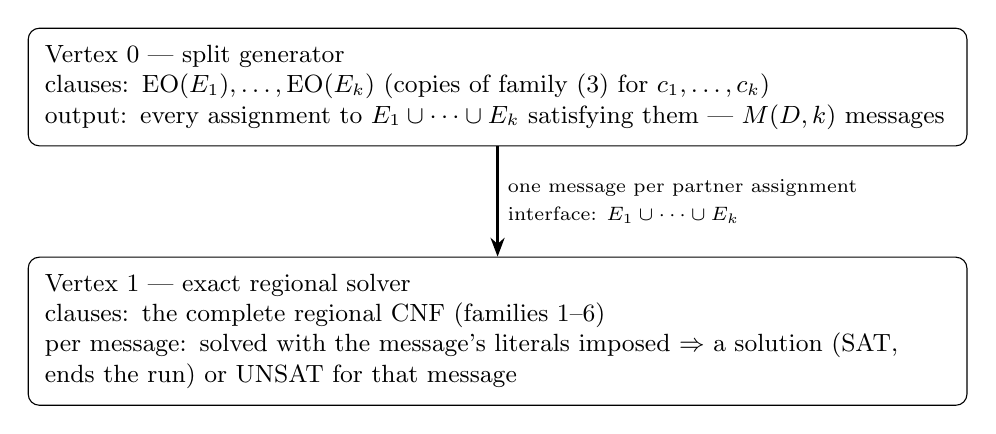
\begin{tikzpicture}[every node/.style={font=\small}, arr/.style={-{Stealth[length=2.4mm]}, thick},
  box/.style={draw, rounded corners, align=left, text width=11.5cm, inner sep=6pt}]
\node[box] (v0) {Vertex 0 --- split generator\\
clauses: $\EO(E_1),\dots,\EO(E_k)$ (copies of family (3) for $c_1,\dots,c_k$)\\
output: every assignment to $E_1\cup\dots\cup E_k$ satisfying them --- $M(D,k)$ messages};
\node[box, below=14mm of v0] (v1) {Vertex 1 --- exact regional solver\\
clauses: the complete regional CNF (families 1--6)\\
per message: solved with the message's literals imposed $\Rightarrow$ a solution
(SAT, ends the run) or UNSAT for that message};
\draw[arr] (v0) -- node[right, align=left]{\scriptsize one message per partner assignment\\[-1pt]
\scriptsize interface: $E_1\cup\dots\cup E_k$} (v1);
\end{tikzpicture}
\caption{The native split DAG. The region is UNSAT-UNCERTIFIED exactly when vertex 0 is
exhausted and every message is UNSAT at vertex 1 with no solution found.}
\label{fig:dag}
\end{figure}

\paragraph{Why the clauses are copied into vertex 0.} Dagster stores one global CNF, and
vertices refer to clauses by index. Vertex 1 must contain the whole regional formula,
including the $\EO$ constraints for $c_1,\dots,c_k$. Appending a second copy of those $\EO$
clauses and giving vertex 0 only the copies makes the source a small, local enumerator,
while the terminal formula stays complete. Duplicate clauses do not change the model set.

\begin{theorem}[Exhaustive disjoint cover]\label{thm:split}
The messages are pairwise distinct assignments to the interface. The sets of regional models
compatible with each message are pairwise disjoint and together cover every model of the
region; some of these sets are empty. Hence the region is UNSAT iff vertex 1 is UNSAT under
every message.
\end{theorem}
\begin{proof}
Let $\pi$ be a model. Each $c_i$ is in exactly one transposition, so $\pi$'s restriction to
$E_1\cup\dots\cup E_k$ satisfies every $\EO(E_i)$ and is enumerated as some message $m$;
$\pi$ is compatible with $m$ and with no other message, since distinct messages differ on an
interface variable. Conversely, a model of vertex 1 under $m$ is a model of the region,
because vertex 1 holds every clause. A message whose literals contradict the matching, for
example two split coordinates choosing the same outside partner, has an empty compatible set
and is refuted at vertex 1 almost at once.
\end{proof}

The theorem holds for any choice of split coordinates and any $k$; the choice affects only
the performance.

\subsection{Number of messages}

Each split coordinate has $D=|V|-1$ potential partners ($D=27$ for $f=4$, $D=29$ for $f=2$).
The constraints $\EO(E_i)$ and $\EO(E_j)$ share exactly one variable, $x_{c_ic_j}$: if $c_i$
chooses $c_j$, both constraints are satisfied by that one variable, so $c_j$ must choose
$c_i$. Vertex 0 contains only these local constraints, not the full matching, so two
unpaired split coordinates may choose the same outside partner. Such messages are generated
deliberately and refuted immediately downstream.

\begin{proposition}\label{prop:M}
The number of messages is
\[
M(D,k)=\sum_{m=0}^{\lfloor k/2\rfloor} N_m(k)\,\bigl(D-(k-1)\bigr)^{k-2m},\qquad
N_m(k)=\frac{k!}{(k-2m)!\,2^m\,m!},
\]
where $N_m(k)$ counts the ways to choose $m$ disjoint pairs among the $k$ split coordinates.
\end{proposition}
\begin{proof}
A message pairs some $m$ disjoint pairs of split coordinates with each other; each of the
remaining $k-2m$ chooses independently among its $D-(k-1)$ partners outside the split set.
\end{proof}

Thus $M(D,2)=(D-1)^2+1$ and $M(D,3)=(D-2)^3+3(D-2)$, giving $M(27,2)=677$,
$M(29,2)=785$ and $M(29,3)=19{,}764$. These are exactly the counts observed in every Dagster
run, and they are re-verified by the audit of Section~\ref{sec:gates}.

\subsection{Unsplit branches and coordinate selection}\label{sec:rule}

A message in which $c_i$ and $c_j$ are paired with each other fixes one transposition among
them instead of two, so it is a subproblem one level shallower than the rest, typically
about an order of magnitude harder. Because a message is never divided across workers, such
an unsplit branch becomes the critical path of the run. If $\{c_i,c_j\}$ is
seed-refuted, the branch is refuted at once (Lemma~\ref{lem:seed}). The selection rule
exploits this.

\begin{figure}[H]
\centering
\begin{minipage}{0.92\linewidth}\small
Algorithm 2 (coordinate selection, \code{dag\_native\_split.py})\label{alg:sel}
\begin{enumerate}[nosep, label=\arabic*.]
\item order $\leftarrow$ \emph{free coordinates} sorted by (partner-domain size, index); all domains
are equal in this encoding, so this is ascending index;
\item $c_1\leftarrow$ first in order; record rule \code{smallest\_domain};
\item for $t=2,\dots,k$: $c_t\leftarrow$ the first coordinate in order, not yet chosen, that is
seed-refuted (Definition~\ref{def:seed}) against every chosen coordinate; record
\code{seed\_refutes\_pairing};
\item if none exists: $c_t\leftarrow\arg\max$ of the number of chosen coordinates against which
it is seed-refuted, ties broken by the earliest position in order; record
\code{fallback\_refutes\_}$r$\code{\_of\_}$t{-}1$, where $r$ is that number;
\item store $(c_1,\dots,c_k)$ and the rules in \code{split\_meta.json}, and copy them into the
result ledger.
\end{enumerate}
\end{minipage}
\end{figure}

\paragraph{Effect on the sample.}
\begin{itemize}
\item $k=2$: a fully seed-refuted $c_2$ exists for all 224 sampled regions with
$f\in\{2,4,6\}$; only the $f=0$ region, which has no fixed points, falls back.
\item $k=3$, $f=2$: two fixed points seed-refute only about 20 of the 435 pairs. No sampled
$f=2$ region has a $c_3$ refuted against both $c_1$ and $c_2$, and only 6 of the 24 contain
three mutually seed-refuted coordinates at all. The fallback picks a $c_3$ refuted against
one of them, leaving $D-2=27$ unsplit branches of depth-2 size among 19{,}764 messages.
\end{itemize}

\subsection{Choice of depth}

The campaign uses depth $k=2$ for $f=4$ (677 messages, about 6.6 per worker) and $k=3$ for
$f=2$ (19{,}764 messages, about 190 per worker). A deeper split makes messages smaller and
shortens the critical path. It can also lower the total work for Dagster's TiniSAT workers,
whose gap to Kissat is small on easy instances and large on hard ones. On $F(\code{R00043})=\{1,13\}$,
going from depth 2 to depth 3 reduced both the wall time (3{,}086\,s to 872\,s) and the
total message work (about 75 to 18 core-hours).

\subsection{Configuration}

\begin{table}[H]
\centering
\begin{tabular}{@{}lll@{}}
\toprule
setting & value & meaning \\
\midrule
\code{-m} & 0 & each worker runs TiniSAT (CDCL) \\
\code{-e} & 0 & enumerate all source solutions; stop at the first full solution \\
\code{-b} & 0 & depth-first allocation of messages \\
\code{-g} & 0 & table-based master \\
MPI ranks & 104 & 1 master + 103 workers, on one 104-core node \\
cap & 3{,}600\,s & per region, campaign default \\
\bottomrule
\end{tabular}
\caption{Dagster configuration. The worker count is $\min(M(D,k),103)$. Mode \code{-e 3}
stops each worker after the first solution per message, which is unsound for exhausting a
multi-vertex DAG; the driver rejects it.}
\label{tab:config}
\end{table}

\subsection{Scheduler behaviour that shapes performance}

These properties, established from Dagster's source, explain the metrics below.
\begin{itemize}
\item \emph{Per-message cost.} A TiniSAT worker builds a fresh copy of vertex 1's clauses and a
new solver for each message, so nothing learned carries over. This costs about 0.1\,s per
message at order 32.
\item \emph{No intra-message parallelism.} One worker solves a message. When fewer messages
remain than idle workers, idle workers receive \emph{copies} of unfinished messages, a
portfolio differing only in solver phase.
\item \emph{Pre-emption.} Workers poll the master every 20{,}000 decisions. If the numbers of
workers on two messages differ by two or more, the master reassigns a busy worker, and its
search on the old message is discarded.
\item \emph{Source duplication.} At the start only the source message exists, so every worker
receives it; with depth-first allocation they move to vertex-1 messages as these appear.
\end{itemize}

\subsection{Instrumentation and metrics}

The master logs, with timestamps, each message it sends to a worker and each report that a
worker has finished. Pairing each send with that worker's next report gives each message's
duration and identifies pre-empted work. The raw master log of every run is kept, compressed.

\begin{table}[H]
\centering
\small
\begin{tabular}{@{}l p{12cm}@{}}
\toprule
\code{msgs} & distinct vertex-1 messages sent, against the upper bound $D^k$ \\
\code{dup} & vertex-1 sends beyond the distinct messages: copies to idle workers, and re-sends \\
\code{start} & time to the first vertex-1 send; below 0.5\,s in every reported run, shown as 0\,s \\
\code{disp} & from then until every vertex-1 message has been sent at least once \\
\code{tail} & from then until the last \emph{completion report}. Duplicate copies still in
flight when the run ends are not waited for \\
\code{longest}, \code{p90} & longest and 90th-percentile completed message duration \\
\code{busy} & total completed message time / (103 workers $\times$ wall time) \\
\code{pre-empt} & mid-message reassignments, and the search time they discarded \\
overhead & wall $-$ (start $+$ disp $+$ tail): MPI launch, 104 processes loading the CNF,
and shutdown \\
\bottomrule
\end{tabular}
\caption{Dagster run metrics.}
\label{tab:metrics}
\end{table}

\subsection{UNSAT acceptance gates}\label{sec:gates}

With no proof and no status line, a Dagster \st{UNSAT-UNCERTIFIED} verdict is accepted only if:
\begin{enumerate}
\item the process exits 0 with an existing, empty solution file, without timeout or a killed rank;
\item the number of distinct vertex-1 messages equals $M(D,k)$ for the recorded split;
\item every distinct message has at least one completion report;
\item every message assigns exactly the interface variables of the recorded split, each once;
\item any worker still holding a message at shutdown holds a copy of a completed one;
\item the CNF, DAG and generator digests match the region and the release.
\end{enumerate}
Gates 2--5 are implemented by \code{hpc/audit\_dagster.py} on the raw master log. Two versions
matter.
\begin{itemize}
\item v1, the version run over the campaign logs on the cluster, checks gate 2, gate 3,
gate 5, and that all messages of a run carry the same \emph{number} of interface literals. Every
run that closed a region passes:
\begin{itemize}
\item the 242 depth-3 $f=2$ runs, $(D,k)=(29,3)$;
\item the depth-2 runs closing R00043 and R00046, $(29,2)$;
\item every $f=4$ depth-2 run, $(27,2)$;
\item all 31 cases of $R_\emptyset$, $(31,3)$.
\end{itemize}
\item v2, released with this report, implements gate 4 in full. It rebuilds the
interface the run actually used, every edge variable incident to the split coordinates recorded
in its ledger, and requires each message to assign exactly those variables, once each. It passes
on the two archived logs examined here (677 of 677 messages match the 53-variable interface) and
fails when given the wrong coordinates.
\end{itemize}
Campaign audit with v2. Run over the archived results, v2 found 317 Dagster runs that
reported UNSAT.
\begin{itemize}
\item 291 have a master log, and every one passes: 244 $f=2$ runs (242 at depth 3, plus
R00043 and R00046 at depth 2), 16 $f=4$ runs, and all 31 cases of $R_\emptyset$.
\item The other 26 have no log. All come from the four earliest jobs, the $f=4$ scaling tests on
R00473, R00621, R01430, R02114, R08990 and R09219, which ran before raw master logs were kept;
the first job to keep them, 181304590, followed directly. All six regions were also closed by
Kissat, and the final inventory credits them to Kissat, so these runs carry no weight.
\end{itemize}
Every region credited to Dagster, and every case, therefore rests on a passing v2 audit
(Section~\ref{app:manifests}).
Logs of runs that ended at their cap fail, as they should. The one exception is R00030's first
run, which passes: its search had in fact finished, and the process was killed during shutdown
(Section~\ref{sec:f2done}).



%======================================================================
\section{Case splitting by a fixed transposition, and symmetry breaking}\label{sec:cases}
The native split relies on fixed points, and one region has none. This section introduces the two devices that close it, a case split on the partner of one coordinate and reflection symmetry breaking, proves both sound, and reports their validation.

%======================================================================

The native split relies on fixed points to refute unsplit branches. The region with no fixed
points, $R_\emptyset$ (\code{R00000}), offers none: no pairing is seed-refuted, the coordinate
rule falls back at every level, and a depth-3 split of the whole region leaves 87 unsplit
branches. In a one-hour run on one node, 84 of the 103 workers spent the entire hour on those
branches and none finished. Two devices remove the problem.

\subsection{Cases on one coordinate's partner}

\begin{theorem}[Case split]\label{thm:case}
For a coordinate $c\in V$, let $R_F^{(c,x)}$ be the set of members of $R_F$ containing the
transposition $(c\,x)$, for $x\in V\setminus\{c\}$. These sets are pairwise disjoint and their
union is $R_F$. Hence $R_F$ is empty iff every $R_F^{(c,x)}$ is empty.
\end{theorem}
\begin{proof}
In any $\pi\in R_F$ the free coordinate $c$ lies in exactly one transposition, $(c\,\pi(c))$.
\end{proof}

A case is encoded by adding the unit clause $x_{cx}$ to the regional CNF, and is written
\code{R00000@0-}$x$ for $c=0$. For $R_\emptyset$ this gives 31 cases, $x=1,\dots,31$.

\paragraph{The fixed transposition is a seed.} Within a case, the two dots $(c,x)$ and $(x,c)$
are known, just as fixed points are known in other regions. Definition~\ref{def:seed} extends
directly: a pairing $\{y,z\}$ is seed-refuted in the case if the dots of $F$, of $(c\,x)$ and of
$(y\,z)$ together repeat a displacement, and Lemma~\ref{lem:seed} applies unchanged.
Algorithm~2 runs with the extended seed and with $c,x$ removed from the candidates. In all 31
cases it finds two coordinates whose pairing is seed-refuted, so a depth-2 split inside any
case has no unsplit branches. No case admits three mutually seed-refuted coordinates, so at
depth 3 about 29 unsplit branches remain per case, now only the size of a depth-2 piece.

\subsection{Reflection symmetry breaking}

\begin{lemma}\label{lem:sb}
Suppose $\rho(F)=F$, where $\rho(i)=n-1-i$. Then $R_F$ is empty iff
$R_F\cap\{\pi:\pi(0)+\pi(n-1)\le n-1\}$ is empty.
\end{lemma}
\begin{proof}
If $\pi\in R_F$, then $\sigma=\rho\pi\rho\in R_F$ by Lemma~\ref{lem:refl}, and
$\sigma(0)+\sigma(n-1)=2(n-1)-(\pi(0)+\pi(n-1))$. So one of $\pi,\sigma$ satisfies the
inequality.
\end{proof}

The constraint is encoded as the binary clauses $\neg h_{0,u}\vee\neg h_{n-1,w}$ for every
pair of permitted images with $u+w>n-1$; at order 32 there are 465. It applies to
$R_\emptyset$, and is combined with the case split. Soundness of the combination follows from
the two results. If $R_\emptyset$ had a member, Lemma~\ref{lem:sb} would give one, $\sigma$,
satisfying the constraint, and $\sigma$ lies in case $x=\sigma(0)$, which would therefore be
satisfiable. Inside case $x$ the constraint is simply $\pi(31)\le31-x$: a direct cut of
coordinate 31's domain, stronger for larger $x$. In case $x=31$, $\pi(31)=0$ is forced and the
constraint removes nothing.

\begin{figure}[H]
\centering
\begin{minipage}{0.47\linewidth}\centering
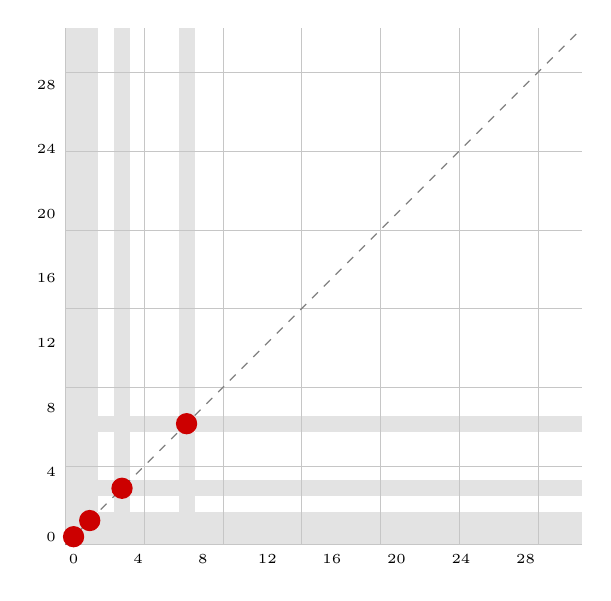
\begin{tikzpicture}[x=0.205cm,y=0.205cm]
\fill[gray!22] (0,1) rectangle (1,2);
\fill[gray!22] (1,0) rectangle (2,1);
\fill[gray!22] (0,2) rectangle (1,3);
\fill[gray!22] (2,0) rectangle (3,1);
\fill[gray!22] (0,3) rectangle (1,4);
\fill[gray!22] (3,0) rectangle (4,1);
\fill[gray!22] (0,4) rectangle (1,5);
\fill[gray!22] (4,0) rectangle (5,1);
\fill[gray!22] (0,5) rectangle (1,6);
\fill[gray!22] (5,0) rectangle (6,1);
\fill[gray!22] (0,6) rectangle (1,7);
\fill[gray!22] (6,0) rectangle (7,1);
\fill[gray!22] (0,7) rectangle (1,8);
\fill[gray!22] (7,0) rectangle (8,1);
\fill[gray!22] (0,8) rectangle (1,9);
\fill[gray!22] (8,0) rectangle (9,1);
\fill[gray!22] (0,9) rectangle (1,10);
\fill[gray!22] (9,0) rectangle (10,1);
\fill[gray!22] (0,10) rectangle (1,11);
\fill[gray!22] (10,0) rectangle (11,1);
\fill[gray!22] (0,11) rectangle (1,12);
\fill[gray!22] (11,0) rectangle (12,1);
\fill[gray!22] (0,12) rectangle (1,13);
\fill[gray!22] (12,0) rectangle (13,1);
\fill[gray!22] (0,13) rectangle (1,14);
\fill[gray!22] (13,0) rectangle (14,1);
\fill[gray!22] (0,14) rectangle (1,15);
\fill[gray!22] (14,0) rectangle (15,1);
\fill[gray!22] (0,15) rectangle (1,16);
\fill[gray!22] (15,0) rectangle (16,1);
\fill[gray!22] (0,16) rectangle (1,17);
\fill[gray!22] (16,0) rectangle (17,1);
\fill[gray!22] (0,17) rectangle (1,18);
\fill[gray!22] (17,0) rectangle (18,1);
\fill[gray!22] (0,18) rectangle (1,19);
\fill[gray!22] (18,0) rectangle (19,1);
\fill[gray!22] (0,19) rectangle (1,20);
\fill[gray!22] (19,0) rectangle (20,1);
\fill[gray!22] (0,20) rectangle (1,21);
\fill[gray!22] (20,0) rectangle (21,1);
\fill[gray!22] (0,21) rectangle (1,22);
\fill[gray!22] (21,0) rectangle (22,1);
\fill[gray!22] (0,22) rectangle (1,23);
\fill[gray!22] (22,0) rectangle (23,1);
\fill[gray!22] (0,23) rectangle (1,24);
\fill[gray!22] (23,0) rectangle (24,1);
\fill[gray!22] (0,24) rectangle (1,25);
\fill[gray!22] (24,0) rectangle (25,1);
\fill[gray!22] (0,25) rectangle (1,26);
\fill[gray!22] (25,0) rectangle (26,1);
\fill[gray!22] (0,26) rectangle (1,27);
\fill[gray!22] (26,0) rectangle (27,1);
\fill[gray!22] (0,27) rectangle (1,28);
\fill[gray!22] (27,0) rectangle (28,1);
\fill[gray!22] (0,28) rectangle (1,29);
\fill[gray!22] (28,0) rectangle (29,1);
\fill[gray!22] (0,29) rectangle (1,30);
\fill[gray!22] (29,0) rectangle (30,1);
\fill[gray!22] (0,30) rectangle (1,31);
\fill[gray!22] (30,0) rectangle (31,1);
\fill[gray!22] (0,31) rectangle (1,32);
\fill[gray!22] (31,0) rectangle (32,1);
\fill[gray!22] (1,0) rectangle (2,1);
\fill[gray!22] (0,1) rectangle (1,2);
\fill[gray!22] (1,2) rectangle (2,3);
\fill[gray!22] (2,1) rectangle (3,2);
\fill[gray!22] (1,3) rectangle (2,4);
\fill[gray!22] (3,1) rectangle (4,2);
\fill[gray!22] (1,4) rectangle (2,5);
\fill[gray!22] (4,1) rectangle (5,2);
\fill[gray!22] (1,5) rectangle (2,6);
\fill[gray!22] (5,1) rectangle (6,2);
\fill[gray!22] (1,6) rectangle (2,7);
\fill[gray!22] (6,1) rectangle (7,2);
\fill[gray!22] (1,7) rectangle (2,8);
\fill[gray!22] (7,1) rectangle (8,2);
\fill[gray!22] (1,8) rectangle (2,9);
\fill[gray!22] (8,1) rectangle (9,2);
\fill[gray!22] (1,9) rectangle (2,10);
\fill[gray!22] (9,1) rectangle (10,2);
\fill[gray!22] (1,10) rectangle (2,11);
\fill[gray!22] (10,1) rectangle (11,2);
\fill[gray!22] (1,11) rectangle (2,12);
\fill[gray!22] (11,1) rectangle (12,2);
\fill[gray!22] (1,12) rectangle (2,13);
\fill[gray!22] (12,1) rectangle (13,2);
\fill[gray!22] (1,13) rectangle (2,14);
\fill[gray!22] (13,1) rectangle (14,2);
\fill[gray!22] (1,14) rectangle (2,15);
\fill[gray!22] (14,1) rectangle (15,2);
\fill[gray!22] (1,15) rectangle (2,16);
\fill[gray!22] (15,1) rectangle (16,2);
\fill[gray!22] (1,16) rectangle (2,17);
\fill[gray!22] (16,1) rectangle (17,2);
\fill[gray!22] (1,17) rectangle (2,18);
\fill[gray!22] (17,1) rectangle (18,2);
\fill[gray!22] (1,18) rectangle (2,19);
\fill[gray!22] (18,1) rectangle (19,2);
\fill[gray!22] (1,19) rectangle (2,20);
\fill[gray!22] (19,1) rectangle (20,2);
\fill[gray!22] (1,20) rectangle (2,21);
\fill[gray!22] (20,1) rectangle (21,2);
\fill[gray!22] (1,21) rectangle (2,22);
\fill[gray!22] (21,1) rectangle (22,2);
\fill[gray!22] (1,22) rectangle (2,23);
\fill[gray!22] (22,1) rectangle (23,2);
\fill[gray!22] (1,23) rectangle (2,24);
\fill[gray!22] (23,1) rectangle (24,2);
\fill[gray!22] (1,24) rectangle (2,25);
\fill[gray!22] (24,1) rectangle (25,2);
\fill[gray!22] (1,25) rectangle (2,26);
\fill[gray!22] (25,1) rectangle (26,2);
\fill[gray!22] (1,26) rectangle (2,27);
\fill[gray!22] (26,1) rectangle (27,2);
\fill[gray!22] (1,27) rectangle (2,28);
\fill[gray!22] (27,1) rectangle (28,2);
\fill[gray!22] (1,28) rectangle (2,29);
\fill[gray!22] (28,1) rectangle (29,2);
\fill[gray!22] (1,29) rectangle (2,30);
\fill[gray!22] (29,1) rectangle (30,2);
\fill[gray!22] (1,30) rectangle (2,31);
\fill[gray!22] (30,1) rectangle (31,2);
\fill[gray!22] (1,31) rectangle (2,32);
\fill[gray!22] (31,1) rectangle (32,2);
\fill[gray!22] (3,0) rectangle (4,1);
\fill[gray!22] (0,3) rectangle (1,4);
\fill[gray!22] (3,1) rectangle (4,2);
\fill[gray!22] (1,3) rectangle (2,4);
\fill[gray!22] (3,2) rectangle (4,3);
\fill[gray!22] (2,3) rectangle (3,4);
\fill[gray!22] (3,4) rectangle (4,5);
\fill[gray!22] (4,3) rectangle (5,4);
\fill[gray!22] (3,5) rectangle (4,6);
\fill[gray!22] (5,3) rectangle (6,4);
\fill[gray!22] (3,6) rectangle (4,7);
\fill[gray!22] (6,3) rectangle (7,4);
\fill[gray!22] (3,7) rectangle (4,8);
\fill[gray!22] (7,3) rectangle (8,4);
\fill[gray!22] (3,8) rectangle (4,9);
\fill[gray!22] (8,3) rectangle (9,4);
\fill[gray!22] (3,9) rectangle (4,10);
\fill[gray!22] (9,3) rectangle (10,4);
\fill[gray!22] (3,10) rectangle (4,11);
\fill[gray!22] (10,3) rectangle (11,4);
\fill[gray!22] (3,11) rectangle (4,12);
\fill[gray!22] (11,3) rectangle (12,4);
\fill[gray!22] (3,12) rectangle (4,13);
\fill[gray!22] (12,3) rectangle (13,4);
\fill[gray!22] (3,13) rectangle (4,14);
\fill[gray!22] (13,3) rectangle (14,4);
\fill[gray!22] (3,14) rectangle (4,15);
\fill[gray!22] (14,3) rectangle (15,4);
\fill[gray!22] (3,15) rectangle (4,16);
\fill[gray!22] (15,3) rectangle (16,4);
\fill[gray!22] (3,16) rectangle (4,17);
\fill[gray!22] (16,3) rectangle (17,4);
\fill[gray!22] (3,17) rectangle (4,18);
\fill[gray!22] (17,3) rectangle (18,4);
\fill[gray!22] (3,18) rectangle (4,19);
\fill[gray!22] (18,3) rectangle (19,4);
\fill[gray!22] (3,19) rectangle (4,20);
\fill[gray!22] (19,3) rectangle (20,4);
\fill[gray!22] (3,20) rectangle (4,21);
\fill[gray!22] (20,3) rectangle (21,4);
\fill[gray!22] (3,21) rectangle (4,22);
\fill[gray!22] (21,3) rectangle (22,4);
\fill[gray!22] (3,22) rectangle (4,23);
\fill[gray!22] (22,3) rectangle (23,4);
\fill[gray!22] (3,23) rectangle (4,24);
\fill[gray!22] (23,3) rectangle (24,4);
\fill[gray!22] (3,24) rectangle (4,25);
\fill[gray!22] (24,3) rectangle (25,4);
\fill[gray!22] (3,25) rectangle (4,26);
\fill[gray!22] (25,3) rectangle (26,4);
\fill[gray!22] (3,26) rectangle (4,27);
\fill[gray!22] (26,3) rectangle (27,4);
\fill[gray!22] (3,27) rectangle (4,28);
\fill[gray!22] (27,3) rectangle (28,4);
\fill[gray!22] (3,28) rectangle (4,29);
\fill[gray!22] (28,3) rectangle (29,4);
\fill[gray!22] (3,29) rectangle (4,30);
\fill[gray!22] (29,3) rectangle (30,4);
\fill[gray!22] (3,30) rectangle (4,31);
\fill[gray!22] (30,3) rectangle (31,4);
\fill[gray!22] (3,31) rectangle (4,32);
\fill[gray!22] (31,3) rectangle (32,4);
\fill[gray!22] (7,0) rectangle (8,1);
\fill[gray!22] (0,7) rectangle (1,8);
\fill[gray!22] (7,1) rectangle (8,2);
\fill[gray!22] (1,7) rectangle (2,8);
\fill[gray!22] (7,2) rectangle (8,3);
\fill[gray!22] (2,7) rectangle (3,8);
\fill[gray!22] (7,3) rectangle (8,4);
\fill[gray!22] (3,7) rectangle (4,8);
\fill[gray!22] (7,4) rectangle (8,5);
\fill[gray!22] (4,7) rectangle (5,8);
\fill[gray!22] (7,5) rectangle (8,6);
\fill[gray!22] (5,7) rectangle (6,8);
\fill[gray!22] (7,6) rectangle (8,7);
\fill[gray!22] (6,7) rectangle (7,8);
\fill[gray!22] (7,8) rectangle (8,9);
\fill[gray!22] (8,7) rectangle (9,8);
\fill[gray!22] (7,9) rectangle (8,10);
\fill[gray!22] (9,7) rectangle (10,8);
\fill[gray!22] (7,10) rectangle (8,11);
\fill[gray!22] (10,7) rectangle (11,8);
\fill[gray!22] (7,11) rectangle (8,12);
\fill[gray!22] (11,7) rectangle (12,8);
\fill[gray!22] (7,12) rectangle (8,13);
\fill[gray!22] (12,7) rectangle (13,8);
\fill[gray!22] (7,13) rectangle (8,14);
\fill[gray!22] (13,7) rectangle (14,8);
\fill[gray!22] (7,14) rectangle (8,15);
\fill[gray!22] (14,7) rectangle (15,8);
\fill[gray!22] (7,15) rectangle (8,16);
\fill[gray!22] (15,7) rectangle (16,8);
\fill[gray!22] (7,16) rectangle (8,17);
\fill[gray!22] (16,7) rectangle (17,8);
\fill[gray!22] (7,17) rectangle (8,18);
\fill[gray!22] (17,7) rectangle (18,8);
\fill[gray!22] (7,18) rectangle (8,19);
\fill[gray!22] (18,7) rectangle (19,8);
\fill[gray!22] (7,19) rectangle (8,20);
\fill[gray!22] (19,7) rectangle (20,8);
\fill[gray!22] (7,20) rectangle (8,21);
\fill[gray!22] (20,7) rectangle (21,8);
\fill[gray!22] (7,21) rectangle (8,22);
\fill[gray!22] (21,7) rectangle (22,8);
\fill[gray!22] (7,22) rectangle (8,23);
\fill[gray!22] (22,7) rectangle (23,8);
\fill[gray!22] (7,23) rectangle (8,24);
\fill[gray!22] (23,7) rectangle (24,8);
\fill[gray!22] (7,24) rectangle (8,25);
\fill[gray!22] (24,7) rectangle (25,8);
\fill[gray!22] (7,25) rectangle (8,26);
\fill[gray!22] (25,7) rectangle (26,8);
\fill[gray!22] (7,26) rectangle (8,27);
\fill[gray!22] (26,7) rectangle (27,8);
\fill[gray!22] (7,27) rectangle (8,28);
\fill[gray!22] (27,7) rectangle (28,8);
\fill[gray!22] (7,28) rectangle (8,29);
\fill[gray!22] (28,7) rectangle (29,8);
\fill[gray!22] (7,29) rectangle (8,30);
\fill[gray!22] (29,7) rectangle (30,8);
\fill[gray!22] (7,30) rectangle (8,31);
\fill[gray!22] (30,7) rectangle (31,8);
\fill[gray!22] (7,31) rectangle (8,32);
\fill[gray!22] (31,7) rectangle (32,8);
\draw[gray!45,very thin] (0,0) grid (32,32);
\draw[gray,dashed] (0,0) -- (32,32);
\fill[red!80!black] (0.5,0.5) circle (0.66);
\fill[red!80!black] (1.5,1.5) circle (0.66);
\fill[red!80!black] (3.5,3.5) circle (0.66);
\fill[red!80!black] (7.5,7.5) circle (0.66);
\node[font=\tiny,below] at (0.5,0) {0};
\node[font=\tiny,left] at (0,0.5) {0};
\node[font=\tiny,below] at (4.5,0) {4};
\node[font=\tiny,left] at (0,4.5) {4};
\node[font=\tiny,below] at (8.5,0) {8};
\node[font=\tiny,left] at (0,8.5) {8};
\node[font=\tiny,below] at (12.5,0) {12};
\node[font=\tiny,left] at (0,12.5) {12};
\node[font=\tiny,below] at (16.5,0) {16};
\node[font=\tiny,left] at (0,16.5) {16};
\node[font=\tiny,below] at (20.5,0) {20};
\node[font=\tiny,left] at (0,20.5) {20};
\node[font=\tiny,below] at (24.5,0) {24};
\node[font=\tiny,left] at (0,24.5) {24};
\node[font=\tiny,below] at (28.5,0) {28};
\node[font=\tiny,left] at (0,28.5) {28};
\end{tikzpicture}
\par\small (a) region $F=\{0,1,3,7\}$
\end{minipage}\hfill
\begin{minipage}{0.47\linewidth}\centering
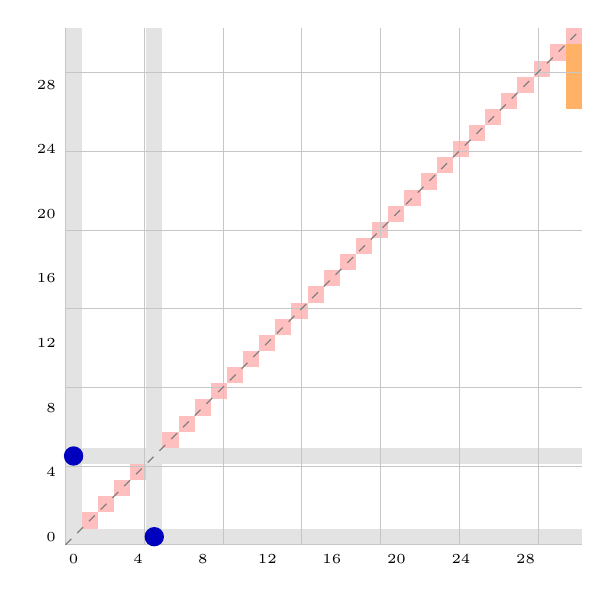
\begin{tikzpicture}[x=0.205cm,y=0.205cm]
\fill[red!25] (0,0) rectangle (1,1);
\fill[red!25] (1,1) rectangle (2,2);
\fill[red!25] (2,2) rectangle (3,3);
\fill[red!25] (3,3) rectangle (4,4);
\fill[red!25] (4,4) rectangle (5,5);
\fill[red!25] (5,5) rectangle (6,6);
\fill[red!25] (6,6) rectangle (7,7);
\fill[red!25] (7,7) rectangle (8,8);
\fill[red!25] (8,8) rectangle (9,9);
\fill[red!25] (9,9) rectangle (10,10);
\fill[red!25] (10,10) rectangle (11,11);
\fill[red!25] (11,11) rectangle (12,12);
\fill[red!25] (12,12) rectangle (13,13);
\fill[red!25] (13,13) rectangle (14,14);
\fill[red!25] (14,14) rectangle (15,15);
\fill[red!25] (15,15) rectangle (16,16);
\fill[red!25] (16,16) rectangle (17,17);
\fill[red!25] (17,17) rectangle (18,18);
\fill[red!25] (18,18) rectangle (19,19);
\fill[red!25] (19,19) rectangle (20,20);
\fill[red!25] (20,20) rectangle (21,21);
\fill[red!25] (21,21) rectangle (22,22);
\fill[red!25] (22,22) rectangle (23,23);
\fill[red!25] (23,23) rectangle (24,24);
\fill[red!25] (24,24) rectangle (25,25);
\fill[red!25] (25,25) rectangle (26,26);
\fill[red!25] (26,26) rectangle (27,27);
\fill[red!25] (27,27) rectangle (28,28);
\fill[red!25] (28,28) rectangle (29,29);
\fill[red!25] (29,29) rectangle (30,30);
\fill[red!25] (30,30) rectangle (31,31);
\fill[red!25] (31,31) rectangle (32,32);
\fill[gray!22] (0,0) rectangle (1,1);
\fill[gray!22] (0,0) rectangle (1,1);
\fill[gray!22] (0,1) rectangle (1,2);
\fill[gray!22] (1,0) rectangle (2,1);
\fill[gray!22] (0,2) rectangle (1,3);
\fill[gray!22] (2,0) rectangle (3,1);
\fill[gray!22] (0,3) rectangle (1,4);
\fill[gray!22] (3,0) rectangle (4,1);
\fill[gray!22] (0,4) rectangle (1,5);
\fill[gray!22] (4,0) rectangle (5,1);
\fill[gray!22] (0,5) rectangle (1,6);
\fill[gray!22] (5,0) rectangle (6,1);
\fill[gray!22] (0,6) rectangle (1,7);
\fill[gray!22] (6,0) rectangle (7,1);
\fill[gray!22] (0,7) rectangle (1,8);
\fill[gray!22] (7,0) rectangle (8,1);
\fill[gray!22] (0,8) rectangle (1,9);
\fill[gray!22] (8,0) rectangle (9,1);
\fill[gray!22] (0,9) rectangle (1,10);
\fill[gray!22] (9,0) rectangle (10,1);
\fill[gray!22] (0,10) rectangle (1,11);
\fill[gray!22] (10,0) rectangle (11,1);
\fill[gray!22] (0,11) rectangle (1,12);
\fill[gray!22] (11,0) rectangle (12,1);
\fill[gray!22] (0,12) rectangle (1,13);
\fill[gray!22] (12,0) rectangle (13,1);
\fill[gray!22] (0,13) rectangle (1,14);
\fill[gray!22] (13,0) rectangle (14,1);
\fill[gray!22] (0,14) rectangle (1,15);
\fill[gray!22] (14,0) rectangle (15,1);
\fill[gray!22] (0,15) rectangle (1,16);
\fill[gray!22] (15,0) rectangle (16,1);
\fill[gray!22] (0,16) rectangle (1,17);
\fill[gray!22] (16,0) rectangle (17,1);
\fill[gray!22] (0,17) rectangle (1,18);
\fill[gray!22] (17,0) rectangle (18,1);
\fill[gray!22] (0,18) rectangle (1,19);
\fill[gray!22] (18,0) rectangle (19,1);
\fill[gray!22] (0,19) rectangle (1,20);
\fill[gray!22] (19,0) rectangle (20,1);
\fill[gray!22] (0,20) rectangle (1,21);
\fill[gray!22] (20,0) rectangle (21,1);
\fill[gray!22] (0,21) rectangle (1,22);
\fill[gray!22] (21,0) rectangle (22,1);
\fill[gray!22] (0,22) rectangle (1,23);
\fill[gray!22] (22,0) rectangle (23,1);
\fill[gray!22] (0,23) rectangle (1,24);
\fill[gray!22] (23,0) rectangle (24,1);
\fill[gray!22] (0,24) rectangle (1,25);
\fill[gray!22] (24,0) rectangle (25,1);
\fill[gray!22] (0,25) rectangle (1,26);
\fill[gray!22] (25,0) rectangle (26,1);
\fill[gray!22] (0,26) rectangle (1,27);
\fill[gray!22] (26,0) rectangle (27,1);
\fill[gray!22] (0,27) rectangle (1,28);
\fill[gray!22] (27,0) rectangle (28,1);
\fill[gray!22] (0,28) rectangle (1,29);
\fill[gray!22] (28,0) rectangle (29,1);
\fill[gray!22] (0,29) rectangle (1,30);
\fill[gray!22] (29,0) rectangle (30,1);
\fill[gray!22] (0,30) rectangle (1,31);
\fill[gray!22] (30,0) rectangle (31,1);
\fill[gray!22] (0,31) rectangle (1,32);
\fill[gray!22] (31,0) rectangle (32,1);
\fill[gray!22] (5,0) rectangle (6,1);
\fill[gray!22] (0,5) rectangle (1,6);
\fill[gray!22] (5,1) rectangle (6,2);
\fill[gray!22] (1,5) rectangle (2,6);
\fill[gray!22] (5,2) rectangle (6,3);
\fill[gray!22] (2,5) rectangle (3,6);
\fill[gray!22] (5,3) rectangle (6,4);
\fill[gray!22] (3,5) rectangle (4,6);
\fill[gray!22] (5,4) rectangle (6,5);
\fill[gray!22] (4,5) rectangle (5,6);
\fill[gray!22] (5,5) rectangle (6,6);
\fill[gray!22] (5,5) rectangle (6,6);
\fill[gray!22] (5,6) rectangle (6,7);
\fill[gray!22] (6,5) rectangle (7,6);
\fill[gray!22] (5,7) rectangle (6,8);
\fill[gray!22] (7,5) rectangle (8,6);
\fill[gray!22] (5,8) rectangle (6,9);
\fill[gray!22] (8,5) rectangle (9,6);
\fill[gray!22] (5,9) rectangle (6,10);
\fill[gray!22] (9,5) rectangle (10,6);
\fill[gray!22] (5,10) rectangle (6,11);
\fill[gray!22] (10,5) rectangle (11,6);
\fill[gray!22] (5,11) rectangle (6,12);
\fill[gray!22] (11,5) rectangle (12,6);
\fill[gray!22] (5,12) rectangle (6,13);
\fill[gray!22] (12,5) rectangle (13,6);
\fill[gray!22] (5,13) rectangle (6,14);
\fill[gray!22] (13,5) rectangle (14,6);
\fill[gray!22] (5,14) rectangle (6,15);
\fill[gray!22] (14,5) rectangle (15,6);
\fill[gray!22] (5,15) rectangle (6,16);
\fill[gray!22] (15,5) rectangle (16,6);
\fill[gray!22] (5,16) rectangle (6,17);
\fill[gray!22] (16,5) rectangle (17,6);
\fill[gray!22] (5,17) rectangle (6,18);
\fill[gray!22] (17,5) rectangle (18,6);
\fill[gray!22] (5,18) rectangle (6,19);
\fill[gray!22] (18,5) rectangle (19,6);
\fill[gray!22] (5,19) rectangle (6,20);
\fill[gray!22] (19,5) rectangle (20,6);
\fill[gray!22] (5,20) rectangle (6,21);
\fill[gray!22] (20,5) rectangle (21,6);
\fill[gray!22] (5,21) rectangle (6,22);
\fill[gray!22] (21,5) rectangle (22,6);
\fill[gray!22] (5,22) rectangle (6,23);
\fill[gray!22] (22,5) rectangle (23,6);
\fill[gray!22] (5,23) rectangle (6,24);
\fill[gray!22] (23,5) rectangle (24,6);
\fill[gray!22] (5,24) rectangle (6,25);
\fill[gray!22] (24,5) rectangle (25,6);
\fill[gray!22] (5,25) rectangle (6,26);
\fill[gray!22] (25,5) rectangle (26,6);
\fill[gray!22] (5,26) rectangle (6,27);
\fill[gray!22] (26,5) rectangle (27,6);
\fill[gray!22] (5,27) rectangle (6,28);
\fill[gray!22] (27,5) rectangle (28,6);
\fill[gray!22] (5,28) rectangle (6,29);
\fill[gray!22] (28,5) rectangle (29,6);
\fill[gray!22] (5,29) rectangle (6,30);
\fill[gray!22] (29,5) rectangle (30,6);
\fill[gray!22] (5,30) rectangle (6,31);
\fill[gray!22] (30,5) rectangle (31,6);
\fill[gray!22] (5,31) rectangle (6,32);
\fill[gray!22] (31,5) rectangle (32,6);
\fill[orange!60] (31,27) rectangle (32,28);
\fill[orange!60] (31,28) rectangle (32,29);
\fill[orange!60] (31,29) rectangle (32,30);
\fill[orange!60] (31,30) rectangle (32,31);
\draw[gray!45,very thin] (0,0) grid (32,32);
\draw[gray,dashed] (0,0) -- (32,32);
\fill[blue!75!black] (0.5,5.5) circle (0.6);
\fill[blue!75!black] (5.5,0.5) circle (0.6);
\node[font=\tiny,below] at (0.5,0) {0};
\node[font=\tiny,left] at (0,0.5) {0};
\node[font=\tiny,below] at (4.5,0) {4};
\node[font=\tiny,left] at (0,4.5) {4};
\node[font=\tiny,below] at (8.5,0) {8};
\node[font=\tiny,left] at (0,8.5) {8};
\node[font=\tiny,below] at (12.5,0) {12};
\node[font=\tiny,left] at (0,12.5) {12};
\node[font=\tiny,below] at (16.5,0) {16};
\node[font=\tiny,left] at (0,16.5) {16};
\node[font=\tiny,below] at (20.5,0) {20};
\node[font=\tiny,left] at (0,20.5) {20};
\node[font=\tiny,below] at (24.5,0) {24};
\node[font=\tiny,left] at (0,24.5) {24};
\node[font=\tiny,below] at (28.5,0) {28};
\node[font=\tiny,left] at (0,28.5) {28};
\end{tikzpicture}
\par\small (b) region $F=\emptyset$, case $(0\,5)$
\end{minipage}
\caption{What a region looks like at order 32. (a) The four fixed points sit on the
diagonal; their rows and columns (grey) cannot hold any other dot, and the other 28
coordinates must be paired into 14 mirror-image transpositions with all displacements
distinct. (b) With no fixed points the diagonal is excluded (red). In case $(0\,5)$ the dots
$(0,5)$ and $(5,0)$ are fixed (blue), and symmetry breaking removes the orange cells:
$\pi(31)\le 26$.}
\label{fig:regions32}
\end{figure}

\subsection{Validation}
\begingroup\sloppy
\begin{itemize}
\item \emph{Symmetry breaking, against brute force.} At orders 8, 10, 12 and 14 every
fixed-point-free Costas involution was enumerated directly: 4, 2, 2 and 4 of them, in mirror
pairs. In every case the CNF has exactly as many models, the CNF with the new clauses has
exactly the number satisfying the constraint (half), and every mirror pair keeps a member.
\item \emph{Case split, at order 10.} The fixed-point-free region has two solutions,
$\pi=(5,9,4,6,2,0,3,8,7,1)$ and its mirror, with $\pi(0)=5$ and $8$. Without symmetry
breaking exactly cases $(0\,5)$ and $(0\,8)$ are SAT; with it only $(0\,5)$ is, through both
Kissat and the native split. All nine case CNFs regenerate to their recorded digests.
\item \emph{Bookkeeping.} A region counts as closed by cases only when, for one coordinate,
every possible partner has an UNSAT case; one missing case leaves it open, and one SAT case
makes it SAT. These three behaviours were tested.
\end{itemize}
\endgroup

%======================================================================
\section{Campaign architecture}\label{sec:campaign}
This section describes how the methods of the preceding sections were organised into a campaign: its stages, the frozen protocol, the scheduling of work, the bookkeeping that tracks every region, and the validation gates passed before results were accepted.

%======================================================================

\subsection{Stages}
\begin{enumerate}
\item Sample. A stratified sample of 225 regions, covering every class, was run with
Kissat for 600\,s, and the timeouts for 4\,h, to measure difficulty before committing the
budget.
\item $f=6$ and $f=4$: Kissat per region. Every remaining region of these classes was
run with Kissat on one core, 104 regions at a time on a node, from a shared queue
(Section~\ref{sec:queue}). The caps were 600\,s for $f=6$ and 3{,}600\,s for $f=4$.
\item $f=4$ stragglers: Dagster, depth 2. The 12 regions Kissat left open after an
hour.
\item $f=2$: Dagster, depth 3, every region. 232 regions in 29 batches of eight,
after the 24 of the sample.
\item $f=0$: case split. The 31 cases of $R_\emptyset$, with symmetry breaking, at
depth 3.
\end{enumerate}

\subsection{Frozen protocol}\label{sec:protocol}
\begin{table}[H]
\centering\small
\begin{tabular}{@{}l p{10.6cm}@{}}
\toprule
item & setting \\
\midrule
region catalogue & \code{regions.csv}, 44{,}947 rows (Algorithm~1; digest in Appendix~\ref{app:digests}) \\
generator & \code{gen\_sym32\_v2.py}, digest \code{59514da058b5e3bc\ldots}, recorded in every ledger \\
Kissat & 4.0.4, one core per region; caps 600\,s ($f=6$), 3{,}600\,s ($f=4$), 4\,h (sample tail) \\
Dagster & AFSAT-Integration commit \code{1c899513\ldots}; flags \code{-m 0 -e 0 -b 0 -g 0}; 104 MPI ranks on one node, 1 master and 103 workers; cap 3{,}600\,s per region or case \\
split depth & 2 for $f=4$; 3 for $f=2$ and for the cases of $R_\emptyset$ \\
coordinates & Algorithm~2, with fixed transpositions as extra seeds in cases \\
symmetry breaking & $\pi(0)+\pi(31)\le31$, for $R_\emptyset$ only \\
accepted verdicts & Section~\ref{sec:solvers}: Kissat exit 20 with \code{s UNSATISFIABLE}; Dagster exit 0 with an empty solution file; any model independently validated \\
audit & Section~\ref{sec:gates}: v1 and then v2 run over every archived master log \\
timeouts and re-runs & a \st{TIMEOUT} never closes a region; re-runs append ledger rows; a region is closed if any accepted verdict exists, and any validated model overrides \\
\bottomrule
\end{tabular}
\caption{The configuration fixed before the class campaigns ran.}
\label{tab:protocol}
\end{table}

\subsection{The shared work queue}\label{sec:queue}
A class batch is one job on one 104-core node. Instead of giving each core a fixed list of
regions in advance, all 104 Kissat processes draw the next region from a common queue. The
queue is a list of ids and a counter on node-local storage, advanced under an exclusive file
lock, so each region is handed out exactly once. The node then stays busy until the work
runs out. The batches used 98--99\% of their allocated CPU time, against the roughly 30\%
waste that fixed lists would cost on $f=4$'s spread of runtimes.

\subsection{Bookkeeping}
\begin{itemize}
\item A status tool scans every result ledger and classifies each region as \st{SAT},
\st{search-closed}, \st{OPEN}, \st{ERROR} or never run.
\item A result counts only if its region identifier exists and its recorded fixed points match
the region table, so test runs cannot pose as campaign results.
\item A region counts as closed by cases only when the cases on one coordinate cover every
possible partner (Theorem~\ref{thm:case}).
\item Every batch job checks, before it ends, that every region it was given has a result, and
fails loudly if not.
\end{itemize}
\subsection{Sampling procedure (\code{hpc/sample.py})}
\begin{itemize}
\item The $f=0$ region is included deterministically.
\item For $f=2,4,6$, the class is sorted by (diameter, region identifier) and cut into four
quartile blocks $g[\,iN/4 : (i+1)N/4\,]$, $i=0,\dots,3$, with integer division.
\item The class quota (24, 100 and 100) is spread as $q/4$ per block, with the first $q\bmod 4$
blocks taking one more.
\item Each block is sampled \emph{without replacement} using Python's \code{random.Random}
seeded with 20261001, a single generator shared across classes in the order $f=2,4,6$.
\item The full list of 225 regions, with their strata, is in
\code{sample\_inventory.csv}. It is
reproduced exactly by re-running the script, and it equals the region set of the Stage-1
ledger.
\end{itemize}
\subsection{Execution in the HPC environment}
\begin{itemize}
\item Single-core work is sharded within a job, each shard pinned to its own core among the
CPUs the job owns. After each job, every selected region must have a result, or the job fails.
\item Region CNFs are generated on node-local storage, solved, and deleted. Only their SHA-256
digests are kept; they are regenerated deterministically on demand.
\item Each result row records: the region and its fixed points; CNF and generator digests;
solver, version and flags; split coordinates and rules; verdict and timings; any witness; and
for Dagster, the master log and the metrics of Table~\ref{tab:metrics}.
\end{itemize}

\subsection{Validation gates passed before results were accepted}
\begin{itemize}
\item the encoding regression suite (Section~\ref{sec:encoding}) reproduced exactly in the HPC environment;
\item Kissat's exit-code behaviour for SAT, UNSAT and time limit was confirmed on login and
compute nodes;
\item an order-10 smoke test, with a known-SAT and a known-UNSAT region, ran every method: all
agreed, and every SAT model was validated;
\item the native split at depths 1, 2 and 3 agreed with Kissat on known regions at orders 10
and 16, including three satisfiable regions. A dropped message would have hidden a solution
there;
\item for the order-32 region $F=\{0,1,3,7\}$, a separate one-coordinate Kissat case split was
machine-checked: the parent formula with all 27 cases negated is UNSAT (coverage), and all
351 pairwise intersections are UNSAT (disjointness).
\end{itemize}



\part{Results}

\section{Results}\label{sec:results}
This section reports the outcome class by class, and ends with the overall result and its accounting by method.


\subsection{Kissat on the sample}

Table~\ref{tab:kissat} gives Stage~1 and the tail. In this sample the fixed-point count is the
strongest observed predictor of runtime. All $f=6$ regions closed within seconds, $f=4$
regions were intermediate, and $f=2$ regions were much harder. Variation within each class
remains material and has not been modelled. Candidate predictors include diameter, the number
of seed-refuted pairs, and the number of unavoidable unsplit branches.

\begin{table}[H]
\centering
\begin{tabular}{@{}rrrrrrr@{}}
\toprule
$f$ & sampled & closed in 600\,s & median & quartiles & max & closed in 4\,h tail \\
\midrule
6 & 100 & 100 & 7.7\,s & 6\,s / 11\,s & 33.9\,s & --- \\
4 & 100 & 78 & 380\,s & 317\,s / 440\,s & 592\,s & 22 of 22 \\
2 & 24 & 0 & --- & --- & --- & 13 of 24 \\
0 & 1 & 0 & --- & --- & --- & 0 of 1 \\
\bottomrule
\end{tabular}
\caption{Kissat on one core. Medians, quartiles and maxima are over regions closed within
600\,s. Every completed run was \st{UNSAT-UNCERTIFIED}, and there were no errors. In the tail,
the $f=4$ regions closed with median 1{,}066\,s and the 13 closed $f=2$ regions with median
11{,}135\,s.}
\label{tab:kissat}
\end{table}

\subsection{Dagster, $f=4$, depth 2}

Two of the hardest $f=4$ regions Kissat closed in Stage~1 were rerun with Dagster, so each
Dagster time has a Kissat baseline.

\begin{table}[H]
\centering
\small
\begin{tabular}{@{}lrrrrrrrrrr@{}}
\toprule
region & Kissat & Dagster & msgs & disp & tail & longest & p90 & busy & wall gain & core cost \\
\midrule
R02114 & 584\,s & 39\,s & 677/729 & 10\,s & 7\,s & 9\,s & 4\,s & 31\% & 15.1$\times$ & 6.9$\times$ \\
R09219 & 592\,s & 37\,s & 677/729 & 9\,s & 5\,s & 9\,s & 4\,s & 30\% & 16.0$\times$ & 6.5$\times$ \\
\bottomrule
\end{tabular}
\caption{$F(\code{R02114})=\{0,7,15,28\}$, $F(\code{R09219})=\{3,7,10,26\}$. Core cost is
$104\times$ the Dagster wall time divided by Kissat's single-core time. Overhead was about 22\,s
in each run.}
\label{tab:f4}
\end{table}

\subsection{Dagster, $f=2$}

All 11 sampled $f=2$ regions that Kissat left open after 4\,h were rerun with Dagster.
Every one was search-closed.

\begin{table}[H]
\centering
\small
\begin{tabular}{@{}lrrrrrrrr@{}}
\toprule
region & depth & wall & disp & tail & longest & p90 & busy & pre-empted \\
\midrule
R00046 & 2 & 2{,}849\,s & 2{,}118\,s & 694\,s & 1{,}071\,s & 665\,s & 85\% & 34{,}378\,s \\
R00043 & 2 & 3{,}086\,s & 2{,}283\,s & 763\,s & 1{,}142\,s & 755\,s & 85\% & 36{,}684\,s \\
\midrule
R00149 & 3 & 277\,s & 250\,s & 5\,s & 99\,s & 3\,s & 91\% & 120\,s \\
R00121 & 3 & 397\,s & 364\,s & 10\,s & 226\,s & 4\,s & 93\% & 420\,s \\
R00097 & 3 & 469\,s & 437\,s & 9\,s & 312\,s & 5\,s & 94\% & 311\,s \\
R00069 & 3 & 611\,s & 576\,s & 11\,s & 493\,s & 6\,s & 95\% & 453\,s \\
R00068 & 3 & 681\,s & 644\,s & 12\,s & 587\,s & 7\,s & 95\% & 500\,s \\
R00254 & 3 & 726\,s & 532\,s & 160\,s & 693\,s & 5\,s & 74\% & 1{,}444\,s \\
R00043 & 3 & 872\,s & 625\,s & 211\,s & 836\,s & 7\,s & 73\% & 10{,}814\,s \\
R00114 & 3 & 882\,s & 846\,s & 14\,s & 684\,s & 10\,s & 96\% & 650\,s \\
R00063 & 3 & 1{,}496\,s & 1{,}243\,s & 217\,s & 1{,}460\,s & 15\,s & 84\% & 9{,}706\,s \\
R00087 & 3 & 2{,}306\,s & 1{,}271\,s & 986\,s & 2{,}257\,s & 12\,s & 57\% & 36{,}084\,s \\
\bottomrule
\end{tabular}
\caption{103 workers. Depth 2 sends 785 messages and depth 3 sends 19{,}764.
$F(\code{R00043})=\{1,13\}$, $F(\code{R00046})=\{1,16\}$. Kissat did not close any of these
regions within 14{,}400\,s.}
\label{tab:f2}
\end{table}
\subsection{The $f=2$ class: complete}\label{sec:f2done}

Besides the 24 sampled regions, the other 232 ran at depth 3 in 29 batches of eight, in region order.
The first five batches, \emph{wave~1}, held R00001--R00040. One region, R00030, reached the 1-hour
cap and was re-run with a 3-hour cap.

\begin{itemize}
\item All 256 $f=2$ regions are \st{search-closed}, and none is satisfiable: 13 by
Kissat within 4\,h, and 243 by Dagster (242 at depth 3, R00046 at depth 2). The cluster's
campaign status reports 256 closed, 0 open, 0 failed and 0 never run.
\item All 192 regions in batches 005--028 closed within the 1-hour cap, the slowest
being $\{1,29\}$ in 2{,}871\,s. R00030 closed on re-run in 3{,}554\,s, making $\{0,30\}$ the
hardest $f=2$ region.
\item Cost: batches 005--028 used 6{,}410 SU, about 33 SU per region, half the wave-1
rate. With wave~1 and R00030's re-run, the campaign used 9{,}212 SU for 232 regions.
\item Audit: every depth-3 master log on the cluster passes gates 2--5.
\end{itemize}

Subject to the claim boundary, this closes one fixed-point class within the present search:
\begin{quote}
\emph{No transpose-symmetric Costas array of order 32 has exactly two fixed points}
(computational, \st{search-closed}; not yet certified).
\end{quote}

\begin{figure}[H]
\centering
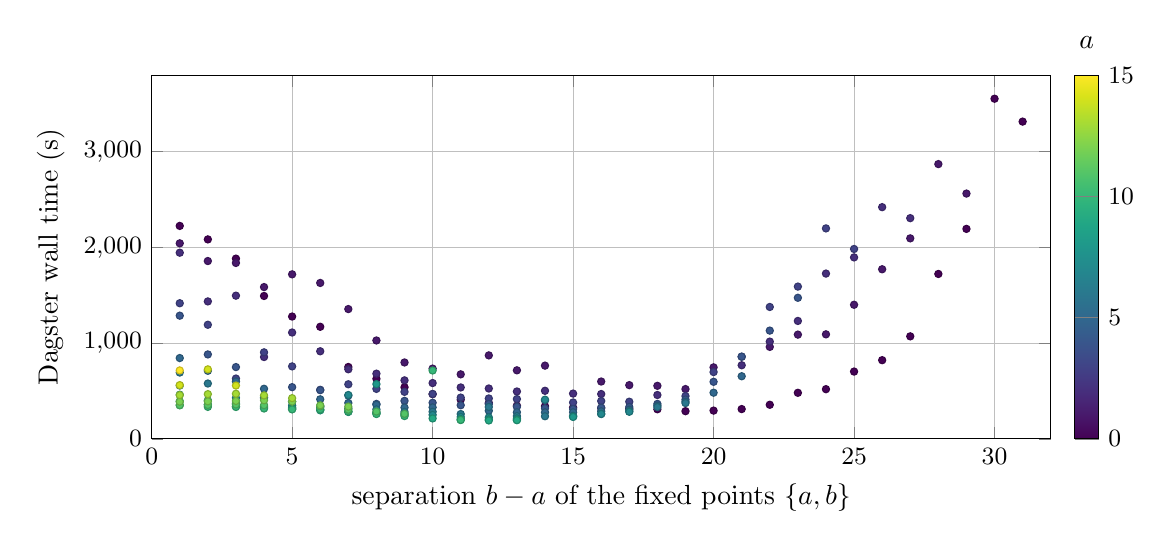
\begin{tikzpicture}
\begin{axis}[width=13cm, height=6.2cm, xlabel={separation $b-a$ of the fixed points $\{a,b\}$},
  ylabel={Dagster wall time (s)}, xmin=0, xmax=32, ymin=0, ymax=3800, grid=major,
  colormap/viridis, colorbar, colorbar style={title={$a$}, width=3mm},
  point meta min=0, point meta max=15, tick label style={font=\small}]
\addplot[scatter, only marks, mark=*, mark size=1.3pt, point meta=explicit] coordinates {(1,2225) [0] (2,2084) [0] (3,1883) [0] (4,1493) [0] (5,1278) [0] (6,1171) [0] (7,751) [0] (8,627) [0] (9,539) [0] (10,467) [0] (11,409) [0] (12,375) [0] (13,347) [0] (14,342) [0] (15,328) [0] (16,321) [0] (17,316) [0] (18,309) [0] (19,289) [0] (20,295) [0] (21,311) [0] (22,356) [0] (23,481) [0] (24,519) [0] (25,703) [0] (26,822) [0] (27,1071) [0] (28,1723) [0] (29,2194) [0] (30,3554) [0] (31,3315) [0] (1,2043) [1] (2,1858) [1] (3,1838) [1] (4,1586) [1] (5,1719) [1] (6,1629) [1] (7,1356) [1] (8,1028) [1] (9,798) [1] (10,734) [1] (11,674) [1] (12,872) [1] (13,716) [1] (14,765) [1] (16,599) [1] (17,561) [1] (18,554) [1] (19,520) [1] (20,747) [1] (22,961) [1] (23,1089) [1] (24,1092) [1] (25,1401) [1] (26,1772) [1] (27,2095) [1] (28,2871) [1] (29,2563) [1] (1,1945) [2] (2,1436) [2] (3,1496) [2] (4,855) [2] (5,1111) [2] (6,915) [2] (7,727) [2] (8,681) [2] (9,611) [2] (10,583) [2] (11,537) [2] (12,526) [2] (13,495) [2] (14,502) [2] (15,473) [2] (16,468) [2] (18,458) [2] (21,769) [2] (22,1016) [2] (23,1232) [2] (24,1727) [2] (25,1896) [2] (26,2421) [2] (27,2306) [2] (1,1417) [3] (2,1192) [3] (3,630) [3] (4,904) [3] (5,757) [3] (6,512) [3] (7,570) [3] (8,522) [3] (9,491) [3] (10,469) [3] (11,431) [3] (12,422) [3] (13,416) [3] (14,402) [3] (15,380) [3] (16,395) [3] (17,388) [3] (19,447) [3] (20,698) [3] (21,858) [3] (22,1378) [3] (23,1591) [3] (24,2199) [3] (25,1984) [3] (1,1287) [4] (2,882) [4] (3,750) [4] (4,428) [4] (5,540) [4] (6,509) [4] (7,452) [4] (8,365) [4] (9,397) [4] (10,377) [4] (11,351) [4] (12,364) [4] (13,335) [4] (14,320) [4] (15,312) [4] (16,326) [4] (17,333) [4] (18,365) [4] (19,411) [4] (20,596) [4] (21,859) [4] (22,1131) [4] (23,1474) [4] (1,844) [5] (2,711) [5] (3,600) [5] (4,523) [5] (5,330) [5] (6,413) [5] (7,375) [5] (8,356) [5] (9,327) [5] (10,329) [5] (12,294) [5] (13,278) [5] (14,277) [5] (15,278) [5] (16,288) [5] (17,305) [5] (18,347) [5] (19,388) [5] (20,482) [5] (21,654) [5] (1,693) [6] (2,578) [6] (4,435) [6] (5,389) [6] (6,341) [6] (7,319) [6] (8,308) [6] (9,282) [6] (10,283) [6] (11,259) [6] (12,333) [6] (13,238) [6] (14,236) [6] (15,240) [6] (16,260) [6] (17,288) [6] (18,332) [6] (19,374) [6] (1,557) [7] (3,428) [7] (5,349) [7] (6,332) [7] (7,458) [7] (8,275) [7] (9,261) [7] (10,250) [7] (11,229) [7] (12,224) [7] (13,214) [7] (14,409) [7] (15,231) [7] (16,260) [7] (17,283) [7] (1,461) [8] (2,402) [8] (3,372) [8] (4,339) [8] (5,320) [8] (6,304) [8] (7,281) [8] (8,572) [8] (9,247) [8] (11,206) [8] (12,203) [8] (13,198) [8] (15,229) [8] (1,392) [9] (2,360) [9] (3,338) [9] (4,326) [9] (5,312) [9] (6,298) [9] (7,285) [9] (8,265) [9] (10,213) [9] (11,197) [9] (12,192) [9] (13,195) [9] (1,351) [10] (2,334) [10] (3,333) [10] (4,317) [10] (5,308) [10] (6,308) [10] (7,286) [10] (8,259) [10] (9,238) [10] (10,714) [10] (11,198) [10] (1,352) [11] (2,354) [11] (3,359) [11] (4,352) [11] (6,340) [11] (7,305) [11] (8,285) [11] (9,261) [11] (1,388) [12] (2,392) [12] (3,396) [12] (4,403) [12] (5,389) [12] (6,350) [12] (7,337) [12] (1,457) [13] (2,467) [13] (3,471) [13] (4,454) [13] (5,425) [13] (1,561) [14] (2,726) [14] (3,557) [14] (1,715) [15]};
\end{axis}
\end{tikzpicture}
\caption{All 242 depth-3 Dagster runs on $f=2$ regions: wall time against the separation of
the two fixed points, coloured by the smaller fixed point $a$. Within each row the shape is
a U shape. Rows with larger $a$ are cheaper and span fewer separations,
since canonical sets satisfy $a+b\le 31$.}
\label{fig:f2all}
\end{figure}

\paragraph{The seven fully split regions.} From the fixed points alone, Algorithm~2 finds three
split coordinates with all pairings seed-refuted in exactly seven $f=2$ regions: R00033,
R00064, R00093, R00120, R00145, R00168 and R00189. These are exactly the seven regions whose
longest message was conspicuously short, 10--52\,s, where comparable regions ran hundreds to
thousands of seconds: none is missing and none is extra. The regions without unsplit branches
are exactly those without long messages. This confirms the account of Section~\ref{sec:rule}:
in this decomposition, unsplit branches set the critical path.

\paragraph{R00030's first run.} That run was recorded \st{TIMEOUT}, yet its master log passes
gates 2--5. Its dispatch (2{,}090\,s) and tail (1{,}488\,s) place the last completed message at
about 3{,}578\,s, so the search had finished before the 3{,}600\,s cap, and the process was
killed during Dagster's shutdown, which took 20--60\,s in every run. Gate~1, normal exit, is what
correctly kept it from being accepted. The re-run then completed normally.

\subsection{The $f=6$ and $f=4$ classes}\label{sec:bulk}

\begin{table}[H]
\centering
\begin{tabular}{@{}lrrrrr@{}}
\toprule
batch & regions & search-closed & timeouts & median & SU \\
\midrule
$f=6$, 000 & 10{,}400 & 10{,}400 & 0 & 13.3\,s & 92.91 \\
$f=6$, 001 & 10{,}400 & 10{,}400 & 0 & 9.7\,s & 66.91 \\
$f=6$, 002 & 10{,}203 & 10{,}203 & 0 & 7.1\,s & 49.05 \\
\midrule
$f=4$, 000 & 2{,}496 & 2{,}486 & 10 & 822\,s & 1{,}372.22 \\
$f=4$, 001 & 2{,}496 & 2{,}494 & 2 & 674\,s & 1{,}098.30 \\
$f=4$, 002 & 2{,}496 & 2{,}496 & 0 & 552\,s & 906.82 \\
$f=4$, 003 & 2{,}496 & 2{,}496 & 0 & 451\,s & 731.76 \\
$f=4$, 004 & 2{,}496 & 2{,}496 & 0 & 359\,s & 545.65 \\
$f=4$, 005 & 1{,}007 & 1{,}007 & 0 & 217\,s & 129.54 \\
\bottomrule
\end{tabular}
\caption{Kissat class batches (one core per region). With the 100 sampled regions of each
class, all 31{,}103 $f=6$ regions are search-closed, and 13{,}575 of the 13{,}587 $f=4$
regions; the other 12 went to Dagster.}
\label{tab:bulk}
\end{table}

Median times fall steadily from batch to batch. Regions are numbered in lexicographic order of
$F$, so the earliest batches hold the sets whose marks start near 0, which pack the fixed
points into one corner of the board. These are hardest, as they are for $f=2$
(Figure~\ref{fig:f2all}).

\paragraph{The 12 $f=4$ stragglers.} All 12 have their four fixed points within a span of 6 to
9, among the most compact four-mark Golomb rulers. Two are the optimal ruler $\{0,1,4,6\}$
and its shift $\{1,2,5,7\}$. For every one of them, Algorithm~2 found a second coordinate whose
pairing with the first is seed-refuted, so the depth-2 split had no unsplit branch. Dagster
closed all 12 in 255--541\,s each (Table~\ref{tab:f4strag}), against more than an hour for
Kissat on one core.

\begin{table}[H]
\centering
\small
\begin{tabular}{@{}llrrrr|llrrrr@{}}
\toprule
region & $F$ & wall & longest & p90 & busy & region & $F$ & wall & longest & p90 & busy \\
\midrule
R00257 & \{0,1,3,7\} & 418 & 247 & 99 & 57\% & R00307 & \{0,1,5,8\} & 266 & 132 & 58 & 56\% \\
R00258 & \{0,1,3,8\} & 334 & 177 & 73 & 56\% & R00608 & \{0,2,3,7\} & 466 & 275 & 108 & 56\% \\
R00259 & \{0,1,3,9\} & 255 & 136 & 60 & 61\% & R00609 & \{0,2,3,8\} & 362 & 181 & 82 & 56\% \\
R00282 & \{0,1,4,6\} & 541 & 299 & 124 & 54\% & R00633 & \{0,2,5,6\} & 494 & 291 & 116 & 54\% \\
R00283 & \{0,1,4,9\} & 259 & 118 & 60 & 56\% & R03729 & \{1,2,5,7\} & 412 & 224 & 96 & 56\% \\
R00306 & \{0,1,5,7\} & 343 & 199 & 82 & 57\% & R04006 & \{1,3,4,8\} & 373 & 207 & 92 & 54\% \\
\bottomrule
\end{tabular}
\caption{The 12 $f=4$ regions Kissat left open, closed by Dagster at depth 2 (times in
seconds; 677 messages each). They used 263 SU in all.}
\label{tab:f4strag}
\end{table}

\subsection{The region with no fixed points}\label{sec:f0}

$R_\emptyset$ was decided through its 31 cases (Section~\ref{sec:cases}), with symmetry
breaking, by Dagster at depth 3: 24{,}476 messages per case, $=M(31,3)$. A depth-2 trial on
cases $(0\,1)$--$(0\,3)$ had first failed to finish in an hour. Every one of its 901 messages
was dispatched, but the 90th-percentile message took about 800\,s. At depth 3, case $(0\,1)$
took 933\,s and about a quarter of the total work, with the 90th percentile at 10\,s, the same
effect of smaller pieces seen on $f=2$.

\begin{figure}[H]
\centering
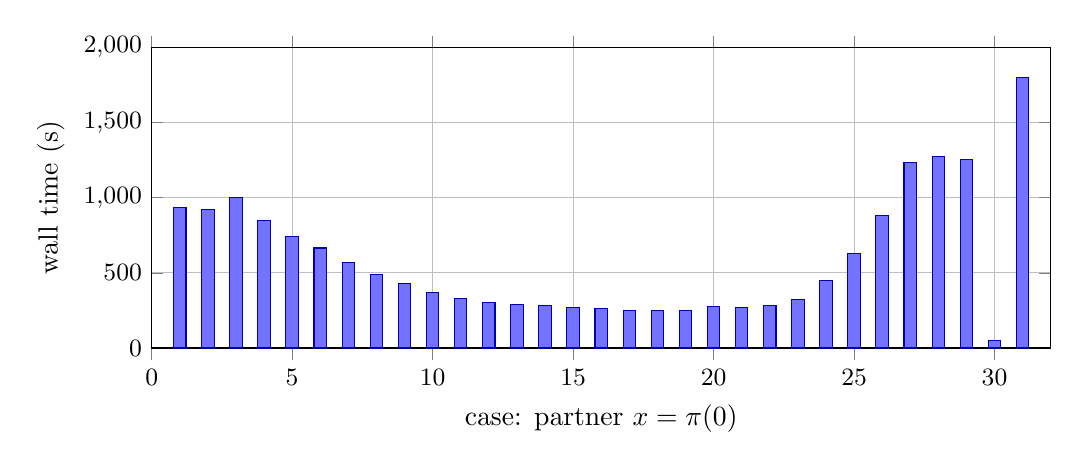
\begin{tikzpicture}
\begin{axis}[width=13cm, height=5.4cm, xlabel={case: partner $x=\pi(0)$},
  ylabel={wall time (s)}, xmin=0, xmax=32, ymin=0, ymax=2000, grid=major, ybar, bar width=4.5pt,
  tick label style={font=\small}]
\addplot[fill=blue!55, draw=blue!70!black] coordinates {(1,933) (2,922) (3,1003) (4,846) (5,742) (6,665) (7,569) (8,491) (9,427) (10,369) (11,331) (12,303) (13,288) (14,281) (15,268) (16,264) (17,249) (18,247) (19,247) (20,278) (21,267) (22,281) (23,321) (24,448) (25,627) (26,882) (27,1232) (28,1271) (29,1254) (30,49) (31,1801)};
\end{axis}
\end{tikzpicture}
\caption{The 31 cases of $R_\emptyset$ (depth 3, 103 workers). Cases 1--23 fall as symmetry
breaking ($\pi(31)\le31-x$) cuts deeper. Cases 24--29 are dominated by one long message
while almost every other piece is trivial: their 90th-percentile message took 0--2\,s.
Case 30 takes 49\,s. In case 31, $\pi(31)=0$ is forced, so symmetry breaking removes
nothing; the transposition $(0\,31)$ is itself mirror-symmetric, so that case still has the full
reflection symmetry.}
\label{fig:f0}
\end{figure}

All 31 cases are \st{UNSAT-UNCERTIFIED}, so $R_\emptyset$ is \st{search-closed}
(Theorem~\ref{thm:case}). The status tool reports \emph{all 31 cases on coordinate 0
$\to$ closed}, and every case log passes the message audit with $(D,k)=(31,3)$. The 31
cases took about 5.1 node-hours and 1{,}057 SU.

\subsection{The result}\label{sec:result}

\begin{table}[H]
\centering
\begin{tabular}{@{}rrrrr@{}}
\toprule
$f$ & regions & closed by Kissat & closed by Dagster & satisfiable \\
\midrule
6 & 31{,}103 & 31{,}103 & --- & 0 \\
4 & 13{,}587 & 13{,}575 & 12 & 0 \\
2 & 256 & 13 & 243 & 0 \\
0 & 1 & --- & 1 (31 cases) & 0 \\
\midrule
all & 44{,}947 & 44{,}691 & 256 & 0 \\
\bottomrule
\end{tabular}
\caption{Every region is \st{search-closed}, confirmed for each class by the status tool on
the cluster. Regions closed by both methods are counted once, under the first method listed.}
\label{tab:final}
\end{table}

\noindent In terms of methods,
\[
\underbrace{44{,}691}_{\text{Kissat}}
+\underbrace{243}_{\text{Dagster, }f=2}
+\underbrace{12}_{\text{Dagster, }f=4}
+\underbrace{1}_{\text{Dagster, 31 cases, }f=0}
=44{,}947 .
\]
The 31 cases are not counted as regions.

\begin{quote}
Computational result. Under the released generator, the exact regional encoding, the
accepted solver rules and the audited execution protocol, all 44{,}947 canonical regions are
\st{search-closed} and no region contains a Costas array. By Theorem~\ref{thm:partition},
\emph{there is no transpose-symmetric Costas array of order 32}. This agrees with the published
enumerations of Section~\ref{sec:censuses}, which the search confirms independently.

Certification status. The negative verdicts are not supported by independently
checked UNSAT proofs. The result is a complete computational exclusion under the trust
assumptions of Section~\ref{sec:claim}, not a formally certified theorem.
\end{quote}

Equivalently: no Costas array of order 32 has any non-trivial symmetry
(Proposition~\ref{prop:onlytranspose}).

\section{Performance analysis}\label{sec:perf}
This section examines where time went in the distributed runs and what the campaign revealed about the decomposition, keeping latency and aggregate cost separate.

%======================================================================

\subsection{Where the wall time goes}
\begin{itemize}
\item \emph{$f=4$, depth 2.} Dispatch takes about 10\,s and the tail 5--7\,s; the longest message
is 9\,s. The other $\approx$22\,s of a 37--39\,s run is overhead, more than half the wall time.
Busy is about 30\%: at this size a full node exceeds what one region needs.
\item \emph{$f=2$, depth 3.} Most regions are throughput-bound, with busy 91--96\% and a tail of
5--14\,s. In R00043, R00063 and R00087 the longest message is almost dispatch plus tail: one
message sets the wall time, almost certainly one of the 27 unsplit branches of depth-2 size
(Section~\ref{sec:rule}). In R00087 that message ran 2{,}257\,s, busy fell to 57\%, and
36{,}084\,s of search was discarded by pre-emption while idle workers raced copies of it.
\end{itemize}

\subsection{Depth}
On R00043, depth 3 cut the wall time 3.5$\times$, the total message work about 4$\times$, and
the pre-empted time 3.4$\times$. The 90th-percentile message fell from 755\,s to 7\,s. The fall
in total work is consistent with TiniSAT keeping pace with Kissat on small instances and falling
behind on large ones; on a 20\,s child of an $f=4$ region the two took 19.8\,s and 19.9\,s.

\subsection{Against Kissat}
For a region taking $T_K$ seconds with Kissat on one core and $T_D$ with Dagster on a
104-core node, the wall-time gain is $T_K/T_D$ and the core-cost ratio is $104\,T_D/T_K$.
Dagster lowers latency on hard regions at an increased aggregate core cost.

\begin{table}[H]
\centering
\begin{tabular}{@{}lrrrr@{}}
\toprule
& Kissat, 1 core & Dagster, 104 cores & wall-time gain & cost \\
\midrule
$f=4$ (R02114, R09219) & 584--592\,s & 37--39\,s & 15--16$\times$ & 6.5--6.9$\times$ core-s \\
$f=2$ hard (10, depth 3) & $>$14{,}400\,s & 277--2{,}306\,s & $>$6--52$\times$ & $\approx$51 SU \\
\bottomrule
\end{tabular}
\caption{For the $f=2$ regions Kissat's true times are unknown beyond 4\,h, so gains are lower bounds.}
\label{tab:vs}
\end{table}

The Dagster configuration measured here gives much lower wall time on the hard regions tested.
The comparison does not isolate the decomposition from the core count or from the
difference between solvers (TiniSAT under Dagster, Kissat alone). Isolating them would need
the same leaf solver run outside Dagster over the same messages. For throughput across many
easy regions, Kissat on one core per region remains cheaper per region.



\subsection{What the decomposition taught}\label{sec:lessons}

\paragraph{Unsplit branches set the critical path.} A message in which two split coordinates
pair with each other is a whole level shallower than the rest. In the $f=2$ class, Algorithm~2
finds a fully seed-refuted triple in exactly seven regions (R00033, R00064, R00093, R00120,
R00145, R00168, R00189). These were exactly the seven regions whose longest message was short,
10--52\,s, while comparable regions ran hundreds to thousands of seconds; none was missing and
none extra. In $R_\emptyset$ at depth 3, without the case split, 84 of the 103 workers spent
the whole hour on unsplit branches. Choosing coordinates whose pairings the seed refutes is
the single most important design rule.

\paragraph{Smaller pieces, less work.} Dagster's TiniSAT workers keep pace with Kissat on
small subproblems but fall behind on large ones. Going one level deeper reduced the
\emph{total} work about fourfold twice: on the $f=2$ region R00043 (about 75 to 18
core-hours), and on case $(0\,1)$ of $R_\emptyset$.

\paragraph{Order matters, structure decides.} Within every class, the compact fixed-point
sets near one corner of the board are the hardest; separations around 20 in the $f=2$ class
are about seven times cheaper. Difficulty is governed by structure, not region size: the
formula sizes within a class vary by only a few per cent.

\subsection{Comparison with a direct search}\label{sec:direct}

The comparisons above are against Kissat on single regions. A more basic question is how the whole
campaign compares with a direct search of the kind used historically, which needs no SAT solver at
all. This project has such a search: a backtracking enumeration of involutions that fixes each
coordinate's partner in turn and rejects repeated displacements incrementally with bitmasks. It
uses the same principle as the Ladendorf midpoint test of the 2009 enumeration, though it is
implemented differently and without symmetry reduction. We timed it on a single 2.8\,GHz Intel Xeon
core of a virtual machine.

\begin{table}[H]
\centering
\begin{tabular}{@{}rrrrrr@{}}
\toprule
order & nodes & ratio & time & arrays & twice the 2009 classes \\
\midrule
16 & 160{,}797 & & 0.05\,s & 40 & 40 \\
18 & 864{,}774 & 5.38 & 0.26\,s & 20 & 20 \\
20 & 4{,}710{,}666 & 5.45 & 1.57\,s & 8 & 8 \\
22 & 25{,}853{,}570 & 5.49 & 9.56\,s & 10 & 10 \\
24 & 142{,}822{,}399 & 5.52 & 58.8\,s & 0 & 0 \\
26 & 791{,}747{,}546 & 5.54 & 382\,s & 4 & 4 \\
\bottomrule
\end{tabular}
\caption{The direct involution search on one core. Node counts agree with those recorded earlier in
the project by three independent implementations. Array counts are exactly twice the 2009 class
counts~\cite{taylor2009}. Ratios are between successive even orders.}
\label{tab:direct}
\end{table}

The node count grows by a factor of about 5.5 per step of two orders, rising slowly, and the time by
about 6.5. Order 32 is three such steps beyond the last measured order. The projection is
about $1.4\times10^{11}$ nodes (between $1.3$ and $1.7\times10^{11}$ for plausible ratios), and 30 to 45
core-hours on this core.

\paragraph{Measured.} The direct search was then run to completion on one 104-core node of our
environment. It was split by the partners of the first three coordinates into 21{,}727 independent tasks,
and preceded by a self-test in which the split reproduced the unsplit search's node and array counts
exactly at orders 16 to 24; at orders 16 to 22 its arrays are also identical, as sorted lists, to those of an
independent unsplit search. Every task completed, and the fail-closed merge found no transpose-symmetric
Costas array of order 32 among $135{,}486{,}910{,}196$ nodes, within $5\%$ of the projection. The search took
$62{,}164$ core-seconds, 17.3 core-hours, and 22 minutes of wall time: faster than projected. It is a
fourth determination of the result, after the enumerations of 1993 and 2009 and the SAT campaign of this
paper, and independent of the last in method and software.

Our campaign's listed production runs used 8{,}443 core-hours (Table~\ref{tab:costs}). For this
problem, then, the direct search needed about 490 times less computation. On latency, it divides
trivially by the partners of the first few coordinates, and on the 104 cores of one node it finished in
22 minutes, against hours of wall time for the campaign. The large gains reported in Table~\ref{tab:vs} are relative to single-core Kissat on the
hardest regions, not to a direct search.

The historical runtime cannot be compared numerically. The 2009 paper reports approximately one year
of processing for its whole extension, covering orders 28 to 36, several symmetry types and the
hardware of the time, without separating order 32. At about $6.5\times$ per two orders, order 36 alone
costs some forty times order 32, so a total of that magnitude is consistent with the measurements
here.

Two conclusions follow.
\begin{itemize}
\item For this problem the decomposition does not save computation. What it adds is an exact
encoding, an audited region-by-region record, and a route to proof certificates. It also offers a
method intended for problems where direct search does not scale, such as structured subclasses of
the general order-32 problem.
\item An earlier projection in this project, $6\times10^{14}$ nodes at order 32 (``a few
core-years''), was wrong. It applied the growth factor once per order rather than once per two orders,
overstating the cost by a factor of about four thousand.
\end{itemize}

\paragraph{Note: latency in search steps, under a common decomposition.}
Suppose the direct search were split into exactly the same pieces as a Dagster run, every piece
had its own processor, and only search steps were counted, ignoring input and output, start-up
and the cost of each step. Both methods would then finish when their hardest piece finishes, so
the comparison comes down to how many steps each needs on a single piece.

\begin{proposition}\label{prop:simulation}
On any piece, a DPLL search on the regional formula, using unit propagation and branching on the
edge variables in the direct search's order, visits a subset of the direct search's nodes.
\end{proposition}
\begin{proof}[Proof sketch]
Every rejection by the direct search is a repeated displacement among placed dots. In the
formula, deciding $x_{cr}$ forces $h_{cr}$ and $h_{rc}$ (clause family~1). With the image literals
of the existing dots true, the indicator clauses (family~5) force the displacement indicator of
each new pair of dots, and a repeated displacement falsifies an at-most-one clause (family~6).
A repeat of a transposition's own displacement $(d,-d)$ is caught the same way, or by the
constraint on transposition lengths (family~4). So each rejection is a propagation conflict at
the same node.
\end{proof}

Counted in steps, then, the SAT solver never needs more than the direct search, and it needs fewer
whenever propagation detects a failure earlier. The main such case is a coordinate left with no
possible partner. A partner whose dots would repeat a displacement has its edge variable propagated
false, and once all are false the coordinate's at-least-one clause fails, before the search ever
branches on that coordinate. Adding exactly this check to the direct search measures how much it
is worth.

\begin{table}[H]
\centering
\begin{tabular}{@{}rrrr@{}}
\toprule
order & nodes, plain & nodes, with the check & reduction \\
\midrule
12 & 5{,}990 & 2{,}312 & 2.6$\times$ \\
14 & 30{,}510 & 10{,}944 & 2.8$\times$ \\
16 & 160{,}797 & 54{,}760 & 2.9$\times$ \\
18 & 864{,}774 & 282{,}811 & 3.1$\times$ \\
20 & 4{,}710{,}666 & 1{,}484{,}965 & 3.2$\times$ \\
\bottomrule
\end{tabular}
\caption{The direct search with and without rejecting any state in which an unmatched coordinate
has no compatible partner. Array counts are identical in both versions.}
\label{tab:wipeout}
\end{table}

The reduction grows ever more slowly, by 0.20, 0.15, 0.12 and then 0.11 per step, which suggests
about $4\times$ at order 32. An exponential separation, of the kind Rintanen established between
SAT-based planning and state-space search~\cite{rintanen2012}, would need failures hidden many levels deep, and the
reduction would then grow geometrically with the order; the data show the hidden failures are
shallow. In steps, therefore, Dagster could finish at most about three or four times sooner than
an equally split direct search: a modest constant factor, not an asymptotic advantage.

In practice the steps do not cost the same. The direct search processes about 2.4 million nodes
per second with bit operations, while each SAT step propagates through a formula of half a million
clauses or more. That difference far exceeds a factor of four, which is why the direct search was
measured as about five hundred times cheaper overall. Even within the direct search, this check
costs more time than it saves at these orders: the run at order 20 takes 2.6 times longer while
visiting a third as many nodes.

Two qualifications apply. The check measures one inference, empty partner domains, which is the
principal one available here; clause learning and the CDCL solver's own branching order lie outside
the proposition and could in principle prune further, although learnt clauses are not shared
between the pieces of a split. And the measurement stops at order 20.


%======================================================================
\section{Cost}\label{sec:cost}
This section accounts for the computational resources the campaign used.

%======================================================================

\begin{table}[H]
\centering
\begin{tabular}{@{}lrl@{}}
\toprule
work & SU & notes \\
\midrule
$f=6$, Kissat & 209 & 3 batches \\
$f=4$, Kissat & 4{,}784 & 6 batches \\
$f=4$, Dagster stragglers & 263 & 12 regions \\
$f=2$, Dagster & 10{,}062 & 243 regions: 11 in the sample, 232 in the campaign \\
$f=0$, Dagster cases & 1{,}057 & 31 cases \\
Kissat tail runs (sample) & 512 & 47 regions at 4\,h \\
\midrule
production total & 16{,}887 & \\
\midrule
exploratory runs & $\approx$1{,}530 & scaling tests, depth trials, the $R_\emptyset$ pilots \\
\bottomrule
\end{tabular}
\caption{Service units in the HPC environment. The listed production runs consumed
16{,}887 SU; the whole research campaign used more, and no complete total is given because
some early and diagnostic runs lack accounting. Charges are about 2 SU per core-hour, on all requested cores for the wall time used. The Stage-1 screen of the sample, the restart sweep and a few early
diagnostic runs are not included; their resource summaries were not recorded.}
\label{tab:costs}
\end{table}

%======================================================================
\section{Claim boundary and trust assumptions}\label{sec:claim}
This section states precisely what the result establishes and what it does not, and lists the assumptions on which it rests.


\paragraph{Relation to the literature.} The non-existence verified here follows from the
exhaustive enumerations of 1993 and 2009 (Section~\ref{sec:censuses}), so
the present work is an independent confirmation, not a first proof. Its value lies in the
independence of the confirmation, since the two methods share no software and no approach, and
in the decomposition that made it possible.

\paragraph{Scope.} The result concerns transpose-symmetric arrays and therefore, by
Proposition~\ref{prop:onlytranspose}, every array invariant under a non-identity motion of the
square. Whether a Costas array of order 32
exists at all remains open.

\paragraph{Two layers.} The \emph{computational result} is that every canonical region is
\st{search-closed} and none contains a validated array. The \emph{certification status} is
that no UNSAT proof has been independently checked. The two are kept separate throughout.

\paragraph{Trust assumptions.} The exclusion assumes that the following are correct:
\begin{itemize}
\item region enumeration and reflection canonicalisation (Algorithm~1, Table~\ref{tab:regions});
\item regional CNF generation (Theorem~\ref{thm:exact});
\item symmetry breaking for $R_\emptyset$ (Lemma~\ref{lem:sb});
\item native-split construction and the case split (Theorems~\ref{thm:split} and~\ref{thm:case});
\item the solvers, Kissat and Dagster's TiniSAT workers;
\item Dagster's message transport and completion accounting;
\item result merging, bookkeeping and the final inventory;
\item file integrity and provenance;
\item the independent model validator (relevant only to SAT results).
\end{itemize}
A SAT witness would be independently checkable. The UNSAT verdicts retain these assumptions
until proofs are produced.

\paragraph{What supports the verdicts.}
\begin{itemize}
\item The encoding is validated exhaustively at orders 8 and 10, and on 158 known arrays.
\item Every decomposition is proved complete.
\item Every Dagster closure passes the message audit (Section~\ref{sec:gates}).
\item Every method reproduced known answers at small orders, including satisfiable regions.
\item Methods agree where both were run.
\item The result is consistent with the earlier structural theorems (Section~\ref{sec:earlier}).
\end{itemize}

%======================================================================
\section{Future work}\label{sec:further}

The computational verification is complete. Three lines of further work suggest themselves, in
increasing distance from the present campaign.

The first is certification. The verdicts reported here rest on the correctness of the solvers and
of our tooling (Section~\ref{sec:claim}). Turning them into a certified result is conceptually
straightforward. Kissat can emit DRAT proofs for the 44{,}691 regions it closed. Each message of a
Dagster split can be materialised as unit clauses on the regional formula and proved in the same
way, so that a region's certificate consists of a checked coverage argument for its split together
with one checked proof per message. The cost at this scale is unknown. It is likely to be
dominated by the hard two-fixed-point regions, and a pilot on a few regions of each class would
settle it. Independently of certification, the released archives should be frozen and hashed, so
that the computational record is fixed.

The second concerns the decomposition. The campaign showed that the native split performs well
exactly when its pieces are small and every unsplit branch is refuted by a seed
(Section~\ref{sec:lessons}). This suggests choosing split coordinates by minimising unsplit
branches over all candidate triples rather than greedily, and refining only the unsplit branches
that remain rather than deepening the whole split. It also invites a more careful evaluation of
Dagster itself, and of the decomposition against direct search, which was far cheaper here. Comparing it with a direct dispatcher over the same split, with the same leaf
solver and across a range of worker counts, would separate the contribution of the decomposition
from those of the solver and the scheduler. It would also quantify the duplicated and discarded
work observed in the tails of runs.

The third is mathematical. The fixed-point partition and the earlier large-large theorems
(Section~\ref{sec:earlier}) approach the same problem from different directions, and together
they may admit a much shorter argument, perhaps one a person could check. The data also show that
regional difficulty is governed by structure: compact rulers packed into one corner of the board
are consistently the hardest. A model of hardness in terms of fixed-point geometry would be of
independent interest, and could guide the decomposition of other structured subclasses at orders
32 and 33, to which the methods here apply with little change. Whether any Costas array of order
32 exists remains beyond these methods.

%======================================================================
\section{Conclusion}

This report revisited the question whether a Costas array of order 32 can be symmetric about its
main diagonal. The question is natural because transpose symmetry is the only symmetry of the
square that a Costas array can have. The literature answers it: exhaustive enumerations published
in 1993 and 2009 find none of order 32. We set out to confirm that answer independently, and to do so with
a method that would carry over to problems that no enumeration reaches.

The approach rests on one structural observation: the fixed points of a transpose-symmetric
Costas array form a Golomb ruler. At order 32 this limits them to 0, 2, 4 or 6, and partitions the
problem into 44{,}947 reflection-canonical regions, each of which can be posed exactly as a
satisfiability problem. Most regions are easy, and a sequential solver closed them. The hard ones
needed a distributed decomposition, and there the same structure proved decisive a second time.
Splitting a region by the partners of a few coordinates works well only if no piece is left in
which two of those coordinates pair with each other, and the fixed points supply exactly the
information needed to refute such pieces in advance. Where there are no fixed points, fixing one
transposition restores the same leverage.

With these devices every region was closed, confirming independently that no transpose-symmetric,
and hence no geometrically symmetric, Costas array of order 32 exists. The confirmation is computational. It is
reproducible from the released software and audited for completeness, but it rests on the
correctness of the solvers and tooling rather than on checked proofs. It is not the cheapest route
to this particular answer: a direct search would have needed far less computation. It agrees with the published enumerations,
and with this project's earlier structural theorems, and it leaves the general order-32 question
open. Its broader lesson is methodological: in a large combinatorial search, the structure that
defines a problem's natural partition can also be made to drive the decomposition of its hardest
parts.

\appendix
\section{Clean-room reproduction}\label{app:repro}
This appendix lists the steps needed to reproduce the campaign from the released software.

\begingroup\sloppy
From an empty directory on a login node of the HPC environment, with the release archive \code{costas32\_hpc.tar.gz}:
\begin{enumerate}[label=\arabic*.]
\item \code{git clone https://github.com/arminbiere/kissat.git; cd kissat; git checkout rel-4.0.4}
(commit \code{8af8e56f\ldots}); \code{./configure \&\& make}; copy \code{build/kissat} to
\code{\$HOME/local/bin}.
\item Build Dagster (AFSAT-Integration branch) against glog 0.4.0, CUDD 3.0.0 and OpenMPI 4.1.0;
apply \code{hpc/patch\_dagster\_wallclock.sh} and build with \code{hpc/build\_dagster.sh}.
\item \code{tar -xzf costas32\_hpc.tar.gz; cd sym32\_sat; source hpc/env.sh}.
\item \code{bash hpc/kissat\_check.sh}, \code{bash hpc/prepare.sh}: this checks the toolchain,
reruns the encoding regression, writes \code{regions.csv} and the 225-region sample, and records
binary digests and versions in \code{\$COSTAS\_DATA/provenance.txt}.
\item \code{qsub hpc/smoke.pbs} (must end \code{SMOKE OK}).
\item \code{qsub hpc/stage1\_kissat.pbs}; then \code{qsub -v STAGE1=\ldots{} hpc/tail\_extend.pbs}.
\item Dagster runs: \code{qsub -v SLOT=104,IDS=\ldots,BASELINE=\ldots,CAP=3600,GRID=\ldots{}
hpc/dagster\_scale.pbs}, with \code{GRID='tini\_d3|3|-m 0 -e 0 -b 0 -g 0'} for $f=2$ and
\code{'tini\_d2|2|\ldots'} for $f=4$.
\item Class campaigns: \code{python3 hpc/campaign.py --f F plan --batch N}; then
\code{F=6 bash hpc/submit\_class.sh} or \code{F=4 bash hpc/submit\_class.sh} (Kissat, shared
queue), or \code{bash hpc/submit\_f2.sh} (Dagster, depth 3). Stragglers:
\code{python3 hpc/campaign.py --f 4 list open} to an id file for \code{hpc/dagster\_scale.pbs}
at depth 2.
\item The $f=0$ region: ids \code{R00000@0-1} \ldots{} \code{R00000@0-31} in an id file, with
\code{qsub -v SYMBREAK=1,SLOT=104,IDS=\ldots,CAP=3600,GRID='tini\_d3|3|-m 0 -e 0 -b 0 -g 0'
hpc/dagster\_scale.pbs}.
\item Status of every class: \code{python3 hpc/campaign.py --f F status} for $F=0,2,4,6$.
\item Checks: \code{verify\_cnf.py} (CNF digests); \code{hpc/audit\_dagster.py} on each master
log; \code{hpc/stage1\_by\_f.py} and \code{hpc/scale\_report.py} regenerate the tables of
Section~\ref{sec:results}.
\end{enumerate}
\endgroup
\section{Manifests and inventories}\label{app:manifests}
This appendix describes the records, made before and after the campaign, that tie its outcome to its artefacts.


\paragraph{Pre-run.} \code{VALIDATION.json} is the frozen manifest written when the encoding was
validated, before the campaign. It is kept unchanged as provenance and is not a campaign summary.
Its generator digest (\code{1bb56e7c\ldots}) predates a later edit that made the order a
parameter. That edit is the identity at order 32, and every campaign ledger records the version
actually run (\code{59514da0\ldots}). All 225 Stage-1 CNFs regenerate byte for byte under that
version.

\paragraph{Post-run.} Two commands on a login node of the HPC environment, with \code{COSTAS\_DATA} set, produce the
authoritative final record from the archived results:
{\footnotesize
\begin{verbatim}
python3 hpc/audit_all.py        # v2 audit of every Dagster closure: audit_results.csv
python3 hpc/final_inventory.py  # final_region_status.csv, f0_cases.csv,
                                 # FINAL_CAMPAIGN_MANIFEST.json
\end{verbatim}}
\begin{itemize}
\item \code{final\_region\_status.csv} has one row per region. Each row gives the final status,
closure method, CNF and generator digests, symmetry breaking, wall time, PBS job, ledger path and
digest, audit result and proof status.
\item A Dagster closure counts only with a passing audit; a region closed by cases counts only if
every case does.
\item R00000's row points to the 31 rows of \code{f0\_cases.csv}.
\item The manifest records the class and method counts, the SAT and not-closed counts (both
required to be zero), the digests of all four files, and the claim level.
\end{itemize}
\paragraph{The final record.} Run on the cluster over the complete results, the two commands
gave:
\begin{itemize}
\item \code{audit\_results.csv}: 317 Dagster runs reporting UNSAT, 291 passing, and 26 without
logs, all early scaling tests on regions also closed by Kissat (Section~\ref{sec:gates});
\item \code{final\_region\_status.csv}: 44{,}947 rows, every one \st{UNSAT-UNCERTIFIED}, namely
1, 256, 13{,}587 and 31{,}103 for $f=0,2,4,6$;
\item closure methods: Kissat 44{,}691; Dagster 255; case split 1 (R00000, 31 cases on
coordinate 0, all \st{UNSAT-UNCERTIFIED});
\item \code{FINAL\_CAMPAIGN\_MANIFEST.json}: SAT-validated 0, not closed 0.
\end{itemize}
The counts in the inventory and the manifest agree with Table~\ref{tab:final}, which was
compiled independently from the job reports. The tools were tested end to end at order 10. A satisfiable region, a Dagster-closed region,
and a case-split region with one satisfiable case were each classified correctly, and deleting a
master log turned its closure into \st{UNAUDITED}.

\section{Reproducing single regions}\label{app:single}
This appendix gives literal commands that reproduce one region of each kind.

On a full compute node, for example in an interactive job, from \code{sym32\_sat}:
{\footnotesize
\begin{verbatim}
source hpc/env.sh; export COSTAS_N=32 DAGSTER_FLAGS="-m 0 -e 0 -b 0 -g 0"
R=$COSTAS_DATA/regions.csv
# a six-fixed-point region with Kissat (about 10 s)
python3 pilot_driver.py --regions $R --ids R20000 --out /tmp/k --arms A --cap 600
python3 verify_cnf.py /tmp/k/ledger.jsonl
# a four-fixed-point straggler with Dagster at depth 2 (about 7 min on 104 cores)
NATIVE_DEPTH=2 python3 pilot_driver.py --regions $R --ids R00257 --out /tmp/d \
    --arms D --ranks 104 --cap 3600
# one case of the fixed-point-free region, with symmetry breaking (about 1 min)
SYMBREAK=1 NATIVE_DEPTH=3 python3 pilot_driver.py --regions $R --ids R00000@0-30 \
    --out /tmp/c --arms D --ranks 104 --cap 3600
# audit that case against the split coordinates its ledger records
C=$(python3 -c "import json
r = json.loads(open('/tmp/c/ledger.jsonl').readlines()[-1])
print(','.join(map(str, r['split_coords'])))")
python3 hpc/audit_dagster.py \
    /tmp/c/dagster_logs/costas_R00000@0-30_*_D.master.log.gz \
    --region R00000@0-30 --depth 3 --coords $C
\end{verbatim}}
Each run must end \st{UNSAT-UNCERTIFIED}, the CNF check must report \code{VERIFY PASS}, and the
audit must report \code{AUDIT PASS}.

\section{Software and digests}\label{app:digests}
This appendix identifies the released software by version and digest.

\begin{table}[H]\centering\footnotesize
\begin{tabular}{@{}l p{5.6cm} l@{}}
\toprule
file & role & SHA-256 (first 24 hex) \\
\midrule
\code{regions.py} & region enumeration & \code{995d949da47783f128430e8d} \\
\code{regions.csv} & its output, 44,947 rows & \code{5710dac9d83e5b277374b568} \\
\code{gen\_sym32\_v2.py} & regional CNF generator & \code{59514da058b5e3bc281c2473} \\
\code{symbreak.py} & reflection symmetry breaking & \code{5b49ce1cae00522625e3530f} \\
\code{dag\_native\_split.py} & native split, Algorithm 2, case splits & \code{47c2713ce95e9532a6c39fb0} \\
\code{pilot\_driver.py} & per-region driver, verdicts, shared queue & \code{ea9ef264d6f740590694c94d} \\
\code{verify\_cnf.py} & CNF digest regeneration & \code{65fd9e1518318cbee9906cad} \\
\code{hpc/run\_shards.sh} & sharding, CPU pinning, completeness check & \code{99821a5747f55602e1e52512} \\
\code{hpc/campaign.py} & class status and planning & \code{6cebb26f6b4553b529b0f9ee} \\
\code{hpc/audit\_dagster.py} & message-accounting audit, v2 & \code{c497651740794962e36e1efc} \\
\code{hpc/audit\_all.py} & audit over every Dagster closure & \code{d1e2ef98cce2dedbaf5cda64} \\
\code{hpc/final\_inventory.py} & final inventory and post-run manifest & \code{b7dfc74a9e4c5b1e1e5f9815} \\
\code{hpc/sample.py} & stratified sample & \code{842ed8e9eefd884786cb48d3} \\
\code{VALIDATION.json} & frozen pre-run validation manifest & \code{5389046124d81fe8197dd7f5} \\
\code{hpc/patch\_dagster\_wallclock.sh} & Dagster wall-clock patch & \code{47cd262eaa78b266672ef2ee} \\
\bottomrule
\end{tabular}
\caption{Digests of the release. The generator digest begins \code{59514da058b5e3bc} and is
recorded in every result ledger.}
\end{table}
\noindent Software: Kissat 4.0.4 (tag \code{rel-4.0.4}, commit
\code{8af8e56f174b778aef3aa45af9f739b2a5f492c2}); Dagster, AFSAT-Integration branch, commit
\code{1c8995131b009410226aa1207d2c622672368293} as recorded in the campaign provenance, built
against glog 0.4.0, CUDD 3.0.0 and OpenMPI 4.1.0, with a patch that only changes its timers to
wall-clock time; Python 3.11. The Dagster commit, binary digests and compiler versions used in the HPC environment are recorded in \code{\$COSTAS\_DATA/provenance.txt}. Nodes: 104 cores and 512\,GB each, 480\,GB requested
per job.
\section{Run log}
This appendix lists the jobs whose results are reported, with their resource use.

\begin{longtable}{@{}lp{7.2cm}rr@{}}
\toprule
job & content & regions & SU \\
\midrule
181301771, 181325004 & Kissat tail runs, 4\,h cap (sample) & 47 & 512.18 \\
181313257 & Dagster $f=4$, depth 2 (R02114, R09219) & 2 & 4.68 \\
181346713 & Dagster $f=2$, depth 2 (R00043, R00046) & 2 & 343.32 \\
181350149 & Dagster $f=2$, depth 3 (R00043) & 1 & 50.73 \\
181352205--07 & Dagster $f=2$, depth 3 (9 sampled regions) & 9 & 455.29 \\
181353964--71 & $f=2$ campaign, batches 000--004 & 40 & 2{,}596.88 \\
181383129--57 & $f=2$ campaign, batches 005--028 & 192 & 6{,}409.71 \\
181383065 & R00030 re-run, 3\,h cap & 1 & 205.63 \\
181449413 & $f=6$ batch 000, Kissat & 10{,}400 & 92.91 \\
181454750--51 & $f=6$ batches 001--002, Kissat & 20{,}603 & 115.96 \\
181449424 & $f=4$ batch 000, Kissat & 2{,}496 & 1{,}372.22 \\
181461103--07 & $f=4$ batches 001--005, Kissat & 10{,}991 & 3{,}412.07 \\
181474613--14 & $f=4$ stragglers, Dagster depth 2 & 12 & 262.66 \\
181474637 & $R_\emptyset$ whole, depth 3, 1\,h cap (exploratory) & 1 & 208.35 \\
181477562 & $R_\emptyset$ cases 1--3, depth 2 (exploratory) & 3 & 624.69 \\
181498459 & $R_\emptyset$ case $(0\,1)$, depth 3 & 1 & 54.25 \\
181499468--71 & $R_\emptyset$ cases 2--31, depth 3 & 30 & 1{,}003.15 \\
\bottomrule
\end{longtable}
\noindent Runs whose results are reported. Stage~1 (job 181257009) and earlier development runs
are omitted.

\section{Supplementary files}
This appendix lists the data files that accompany the report.

\begingroup\sloppy
\begin{itemize}
\item \code{sample\_inventory.csv}: the 225 sampled regions, with stratum, CNF digest, the
historical Stage-1 outcome, and the final method and status of each. R00000 records its 31-case
closure.
\item \code{f2\_campaign\_all.csv}: all 256 $f=2$ regions, with fixed points, separation, method,
Dagster depth, wall time and PBS job.
\item \code{f2\_campaign\_wave1.csv}: per-message metrics for R00001--R00040.
\item \code{costas32\_hpc.tar.gz}: every script named in this report, including
\code{VALIDATION.json}.
\item Generated on the cluster from the campaign results (Appendix~\ref{app:manifests}):
\code{audit\_results.csv}, \code{final\_region\_status.csv} (44{,}947 rows),
\code{f0\_cases.csv} (31 rows) and \code{FINAL\_CAMPAIGN\_MANIFEST.json}.
\end{itemize}
\endgroup

\begin{thebibliography}{99}
\bibitem{costas1984}
J.~P. Costas, A study of a class of detection waveforms having nearly ideal range--Doppler
ambiguity properties, \emph{Proc.\ IEEE} 72(8):996--1009, 1984.
\bibitem{golombtaylor1984}
S.~W. Golomb and H.~Taylor, Constructions and properties of Costas arrays, \emph{Proc.\ IEEE}
72(9):1143--1163, 1984.
\bibitem{drakakis2006}
K.~Drakakis, A review of Costas arrays, \emph{Journal of Applied Mathematics}, 2006.
\bibitem{drakakis2011}
K.~Drakakis, F.~Iorio, S.~Rickard and J.~Walsh, Results of the enumeration of Costas arrays of
order 29, \emph{Advances in Mathematics of Communications} 5(3):547--553, 2011.
\bibitem{taylor2009}
K.~Taylor, S.~Rickard and K.~Drakakis, On Costas arrays with various types of symmetry,
\emph{16th International Conference on Digital Signal Processing}, 2009,
doi:10.1109/ICDSP.2009.5201135.
\bibitem{dgo2006}
K.~Drakakis, R.~Gow and L.~O'Carroll, On some properties of Costas arrays generated via finite
fields, \emph{40th Annual Conference on Information Sciences and Systems}, 801--805, 2006.
\bibitem{brown1993}
C.~Brown, M.~Cenki, R.~Games, J.~Rushanan, O.~Moreno and P.~Pei, New enumeration results for
Costas arrays, \emph{IEEE International Symposium on Information Theory}, 405, 1993.
\bibitem{rintanen2012}
J.~Rintanen, Planning as satisfiability: heuristics, \emph{Artificial Intelligence} 193:45--86, 2012.
\bibitem{kissat}
A.~Biere, K.~Fazekas, M.~Fleury and M.~Heisinger, CaDiCaL, Kissat, Paracooba, Plingeling and
Treengeling entering the SAT Competition 2020, \emph{Proc.\ SAT Competition 2020}, 2020.
\bibitem{dagster}
Dagster: distributed SAT solving over DAG decompositions, \url{https://github.com/ANU-HPC/dagster}.
\bibitem{drattrim}
N.~Wetzler, M.~J.~H. Heule and W.~A. Hunt, DRAT-trim: efficient checking and trimming using
expressive clausal proofs, \emph{SAT 2014}, LNCS 8561, 2014.
\end{thebibliography}
\end{document}
